There are many aspects to evaluation of a software project. In this section we
cover the most important factors. First we asses whether the overall goal of the
project has been reached, whether it solves the problems that we have
addressed. Disregarding the intention of the project we then look at how it
performs compared to other abstract machine implementation, namely JVM and
CIL. We then look at the architectural design in retrospect and determines
whether there were any fundamental design flaws that we would or should have
differently. We then go into the technical details of the system and describe
the process by which we have performed performance measurements and
corresponding optimization.

\subsection{Paradigm Support}

The initial goal of the project was to implement an abstract machine more
suitable for modern language paradigms than the popular contemporary
solutions. Contained in this is the obvious challenge of actually implementing
an abstract machine from scratch with all the bells and whistles required.

To begin with we would like to stress the fact that we did not design the
specification for \thename{}. We have been in close collaboration with our
advisor Sven Karlsson who have done the all the concrete writing of it.

A fundamental aspect of the design of \thename{} is that it exposes primitives
that a compiler can use to construct a run-time system suitable for the language
at hand. We believe this has been accomplished to a large extent.

The concept of an \code{AnyType} capable of expressing arbitrary values can make
code generation for dynamic languages much easier because variables do not have
to declare their type and because the type can change during run-time. Composite
types are similarly dynamic in the sense that members can be added and removed
on demand which is common for many dynamic languages. It also provides easy
dynamic dispatch because \thename{} automatically can look up a sub-routine
member by name.

One of the most powerful features of \thename{} is the fact that at its core it
is very simple and flexible which makes it capable of expressing many language
features by combining the provided building blocks in various ways. There are
few restrictions as to how the primitives can be used.

As for functional language support, the way sub-routines work could be a
significant improvement. In JVM and CIL a sub-routine \emph{must} be attached to
an object, but \thename{} allows sub-routines to exists by themselves and can be
loaded and executed from anywhere facilitation first-class functions. The
execution context can be controlled by managing the use of scopes, something
that the compiler is free to do how it sees fit.

The current implementation is not mature enough to be a sensible target for code
generation, but it does serve as a proof-of-concept that the fundamental ideas
work and could be made production ready. A serious effort could result in a
significant improvement to what is otherwise available.

\subsection{Performance Analysis}
\label{sec:eval:performance}

When analyzing performance, results are relative to other implementations, as
this gives natural standpoint on what is considered good performance, and what
is considered bad. In our case it would be natural to compare the performance of
\thename{} to related work on stack based abstract machines. Here we have chosen
the previously mentioned Java Virtual Machine and Microsoft's Common Language
Runtime.

To make the the results of such a comparison as valuable as possible, it is
beneficial to focus on isolated functionality, as there are many wheels turning
in a such a big piece of software. If one casts the net too wide, it can be
difficult to interpret what results are indicating. Even though JVM and CLR are
both stack machines, they have characteristics which distinguish them and makes
them difficult to directly compare.

We will therefore perform analysis through so-called micro benchmarking, which
as opposed to benchmarking in general, focuses on isolated components or
specific functionality.

\subsubsection{Micro Benchmarking}

One way of creating benchmarks would be to write small programs, as similar as
possible, in programming languages which each has a front-end for the given
machine. For instance, we could write source code in Java to run on JVM and C\#
to run on CLR. The problem with this is that we cannot be sure of what code the
compiler produces. Two very similar programs in each of these two languages,
could likely be compiled to very different byte code. To address this issue, we
disassembled the compiled code to each of the machine's intermediate languages,
namely Java Bytecode and CIL. From the disassembled code we analyzed which
instructions each compiler emitted and in cases where they differed
substantially, we manually altered them and assemble them back to an executable.

Having two executables, one for JVM and one for CLR, and a \thename{} test
program, which we are satisfied with being as similar as possible, we start
measuring their performance. We ran the tests through automated shell scripts
that measured the execution time for a set of parameters for each machine. To
make sure we did not get sporadic results caused by other processes running on
the host machine, we ran each benchmark of each machine over several
rounds. From this we calculated the mean running time for each parameter on each
machine.

We have picked four different cases that we wish to measure, namely stack
operations, recursion, sub-routine invocation and field operations on heap
object. We will go through each in turn, analyzing the results.

% stack

To benchmark the stack we made a simple program which essentially just does a
lot of trivial stack operations. A simple way to achieve this was to take a
large number and decrement it until it becomes zero.

\begin{stackops}
  \op{large pushLiteral i32 n}{n}
  \op{pushLiteral i32 1}{n,\ 1}
  \op{pushElement 1}{n,\ 1,\ n}
  \op{sub}{n,\ (n-1)}
  \op{pushElement 0}{n,\ (n-1),\ (n-1)}
  \op{storeElement 2}{(n-1),\ (n-1)}
  \op{cmpZero}{(n-1),\ b}
  \op{brFalse -13}{(n-1)}
  \op{halt}{-}
\end{stackops}

This induces 9 stack operation per iteration, plus the initial one, which
equals $9n + 1$, where $n = 1\ ...\ (2^{31} -1)$, giving the complexity of
$O(n)$. CIL does not have an \instr{storeElement} instruction, but achieves the
same effect by storing the value in a local variable and then loading it again,
done with {\tt stloc} and {\tt ldloc} (store / load local variable).

The result can be seen in the seen below, in
Figure~\ref{fig:eval:benchmark:stack}.
\begin{figure}[H]
  \centering
  \scalebox{0.8}[0.6]{% Created by tikzDevice version 0.8.1 on 2015-06-28 16:16:19
% !TEX encoding = UTF-8 Unicode
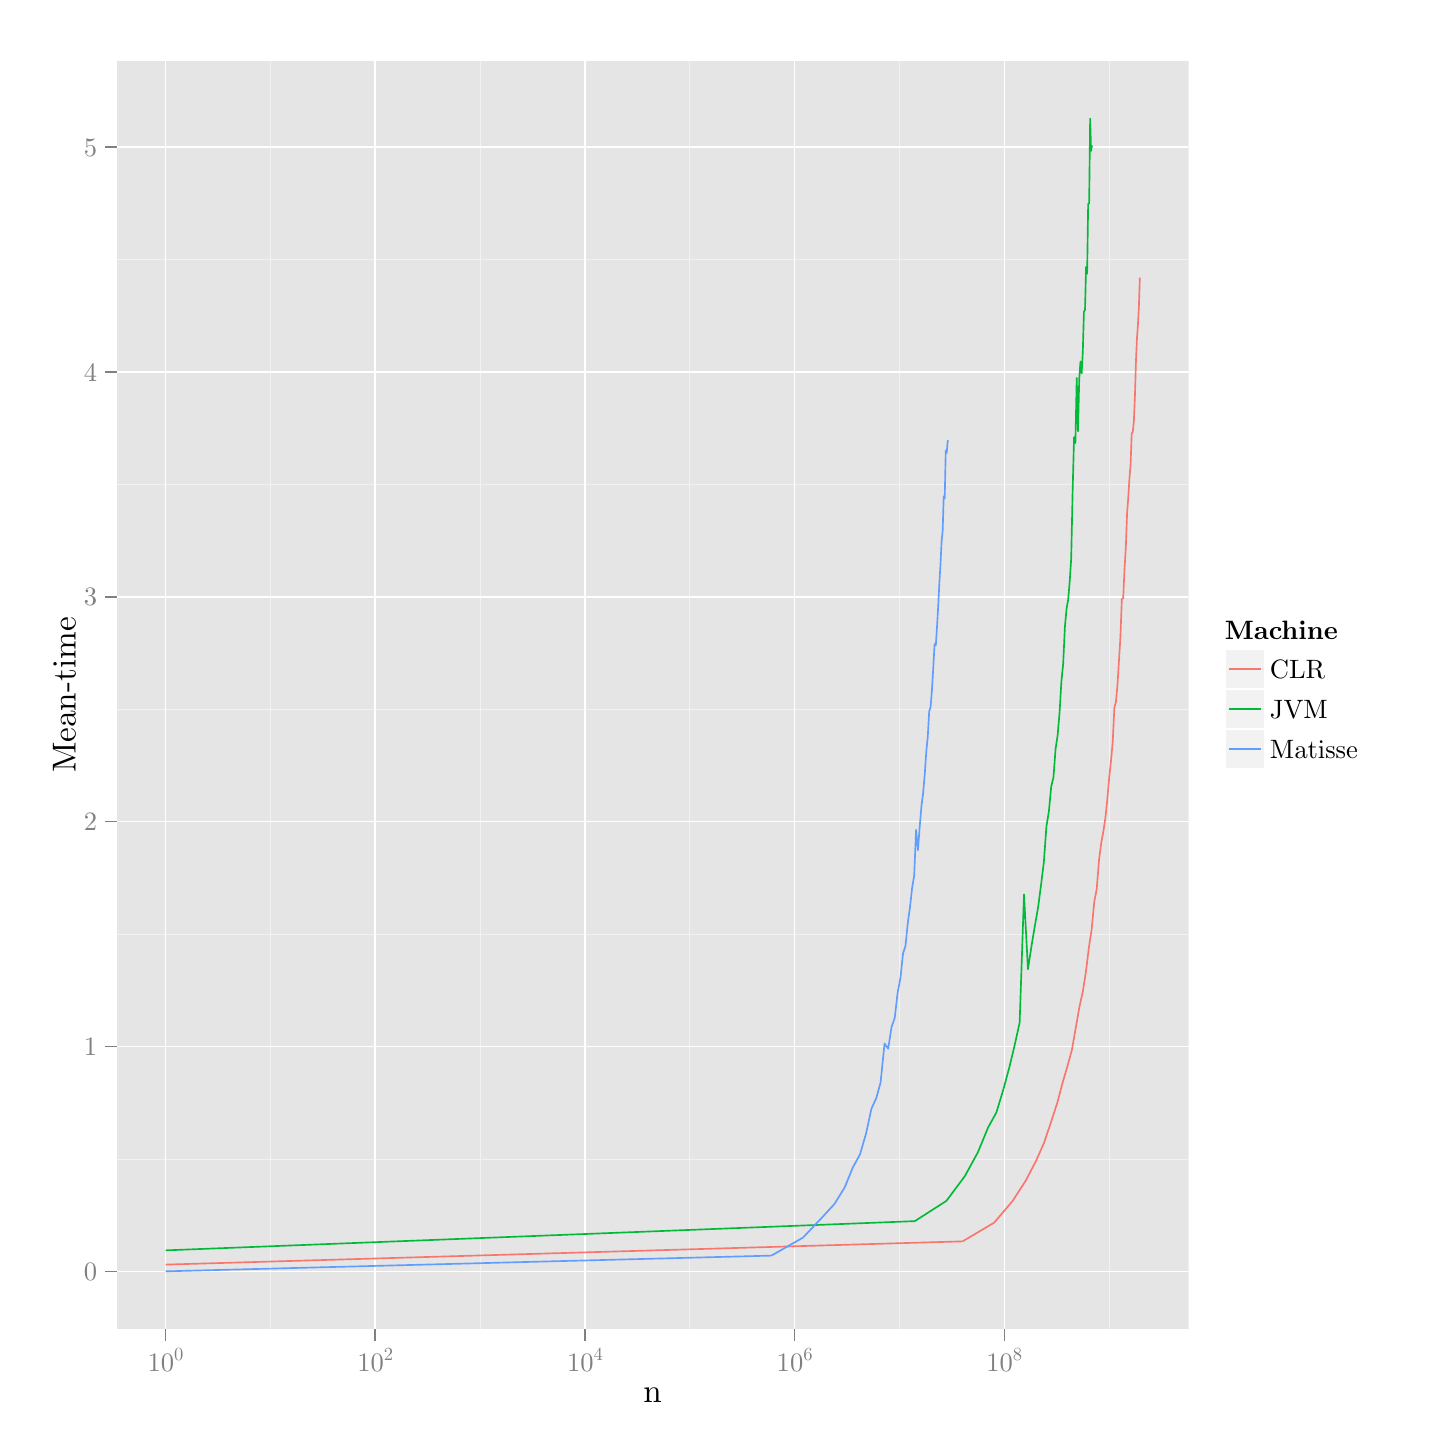
\begin{tikzpicture}[x=1pt,y=1pt]
\definecolor{fillColor}{RGB}{255,255,255}
\path[use as bounding box,fill=fillColor,fill opacity=0.00] (0,0) rectangle (505.89,505.89);
\begin{scope}
\path[clip] (  0.00,  0.00) rectangle (505.89,505.89);
\definecolor{drawColor}{RGB}{255,255,255}
\definecolor{fillColor}{RGB}{255,255,255}

\path[draw=drawColor,line width= 0.6pt,line join=round,line cap=round,fill=fillColor] (  0.00,  0.00) rectangle (505.89,505.89);
\end{scope}
\begin{scope}
\path[clip] ( 32.22, 35.66) rectangle (419.48,493.85);
\definecolor{fillColor}{gray}{0.90}

\path[fill=fillColor] ( 32.22, 35.66) rectangle (419.48,493.85);
\definecolor{drawColor}{gray}{0.95}

\path[draw=drawColor,line width= 0.3pt,line join=round] ( 32.22, 97.11) --
	(419.48, 97.11);

\path[draw=drawColor,line width= 0.3pt,line join=round] ( 32.22,178.36) --
	(419.48,178.36);

\path[draw=drawColor,line width= 0.3pt,line join=round] ( 32.22,259.61) --
	(419.48,259.61);

\path[draw=drawColor,line width= 0.3pt,line join=round] ( 32.22,340.85) --
	(419.48,340.85);

\path[draw=drawColor,line width= 0.3pt,line join=round] ( 32.22,422.10) --
	(419.48,422.10);

\path[draw=drawColor,line width= 0.3pt,line join=round] ( 87.71, 35.66) --
	( 87.71,493.85);

\path[draw=drawColor,line width= 0.3pt,line join=round] (163.48, 35.66) --
	(163.48,493.85);

\path[draw=drawColor,line width= 0.3pt,line join=round] (239.26, 35.66) --
	(239.26,493.85);

\path[draw=drawColor,line width= 0.3pt,line join=round] (315.03, 35.66) --
	(315.03,493.85);

\path[draw=drawColor,line width= 0.3pt,line join=round] (390.81, 35.66) --
	(390.81,493.85);
\definecolor{drawColor}{RGB}{255,255,255}

\path[draw=drawColor,line width= 0.6pt,line join=round] ( 32.22, 56.49) --
	(419.48, 56.49);

\path[draw=drawColor,line width= 0.6pt,line join=round] ( 32.22,137.73) --
	(419.48,137.73);

\path[draw=drawColor,line width= 0.6pt,line join=round] ( 32.22,218.98) --
	(419.48,218.98);

\path[draw=drawColor,line width= 0.6pt,line join=round] ( 32.22,300.23) --
	(419.48,300.23);

\path[draw=drawColor,line width= 0.6pt,line join=round] ( 32.22,381.48) --
	(419.48,381.48);

\path[draw=drawColor,line width= 0.6pt,line join=round] ( 32.22,462.73) --
	(419.48,462.73);

\path[draw=drawColor,line width= 0.6pt,line join=round] ( 49.82, 35.66) --
	( 49.82,493.85);

\path[draw=drawColor,line width= 0.6pt,line join=round] (125.60, 35.66) --
	(125.60,493.85);

\path[draw=drawColor,line width= 0.6pt,line join=round] (201.37, 35.66) --
	(201.37,493.85);

\path[draw=drawColor,line width= 0.6pt,line join=round] (277.14, 35.66) --
	(277.14,493.85);

\path[draw=drawColor,line width= 0.6pt,line join=round] (352.92, 35.66) --
	(352.92,493.85);
\definecolor{drawColor}{RGB}{248,118,109}

\path[draw=drawColor,line width= 0.6pt,line join=round] ( 49.82, 58.92) --
	(337.84, 67.32) --
	(349.25, 74.09) --
	(355.92, 81.94) --
	(360.65, 89.26) --
	(364.32, 96.30) --
	(367.32,103.07) --
	(369.86,110.65) --
	(372.06,117.42) --
	(373.99,124.73) --
	(375.73,130.69) --
	(377.30,136.38) --
	(378.73,144.50) --
	(380.05,152.09) --
	(381.26,157.50) --
	(382.40,164.82) --
	(383.46,173.48) --
	(384.46,179.98) --
	(385.40,190.00) --
	(386.29,194.61) --
	(387.13,205.17) --
	(387.94,211.40) --
	(388.70,215.46) --
	(389.43,220.34) --
	(390.13,227.11) --
	(390.81,234.96) --
	(391.45,240.92) --
	(392.07,247.69) --
	(392.67,260.15) --
	(393.25,262.31) --
	(393.81,268.54) --
	(394.34,277.21) --
	(394.87,285.88) --
	(395.37,299.42) --
	(395.86,299.69) --
	(396.34,310.25) --
	(396.80,317.83) --
	(397.26,330.29) --
	(397.69,335.98) --
	(398.12,343.02) --
	(398.54,348.17) --
	(398.94,359.27) --
	(399.34,359.81) --
	(399.73,363.88) --
	(400.11,373.08) --
	(400.48,385.54) --
	(400.84,393.67) --
	(401.19,398.54) --
	(401.54,405.31) --
	(401.88,415.60);
\definecolor{drawColor}{RGB}{0,186,56}

\path[draw=drawColor,line width= 0.6pt,line join=round] ( 49.82, 64.07) --
	(320.57, 74.63) --
	(331.97, 81.94) --
	(338.64, 90.88) --
	(343.38, 99.55) --
	(347.05,108.48) --
	(350.05,113.90) --
	(352.59,122.30) --
	(354.78,130.42) --
	(356.72,138.55) --
	(358.45,146.40) --
	(360.02,192.71) --
	(361.45,165.63) --
	(362.77,174.30) --
	(363.99,181.61) --
	(365.13,188.11) --
	(366.19,196.23) --
	(367.19,204.36) --
	(368.13,217.36) --
	(369.02,222.77) --
	(369.86,231.71) --
	(370.66,234.96) --
	(371.43,245.25) --
	(372.16,250.13) --
	(372.86,258.25) --
	(373.53,269.63) --
	(374.18,276.13) --
	(374.80,289.40) --
	(375.40,295.90) --
	(375.97,299.15) --
	(376.53,305.65) --
	(377.07,314.04) --
	(377.59,338.15) --
	(378.10,357.92) --
	(378.59,355.75) --
	(379.07,379.31) --
	(379.53,360.08) --
	(379.98,379.04) --
	(380.42,385.27) --
	(380.85,380.94) --
	(381.26,388.52) --
	(381.67,403.14) --
	(382.07,403.96) --
	(382.45,419.39) --
	(382.83,416.96) --
	(383.20,442.14) --
	(383.56,442.41) --
	(383.92,473.02) --
	(384.26,461.37) --
	(384.60,463.27);
\definecolor{drawColor}{RGB}{97,156,255}

\path[draw=drawColor,line width= 0.6pt,line join=round] ( 49.82, 56.49) --
	(268.74, 62.17) --
	(280.14, 68.67) --
	(286.82, 75.71) --
	(291.55, 80.86) --
	(295.22, 86.82) --
	(298.22, 94.13) --
	(300.76, 98.74) --
	(302.95,106.32) --
	(304.89,115.26) --
	(306.63,119.05) --
	(308.19,124.73) --
	(309.63,138.82) --
	(310.94,136.92) --
	(312.16,144.78) --
	(313.30,148.03) --
	(314.36,157.23) --
	(315.36,162.38) --
	(316.30,171.32) --
	(317.19,174.03) --
	(318.03,182.42) --
	(318.83,188.11) --
	(319.60,195.15) --
	(320.33,199.48) --
	(321.03,216.00) --
	(321.70,208.69) --
	(322.35,217.36) --
	(322.97,224.67) --
	(323.57,229.27) --
	(324.15,236.04) --
	(324.70,244.17) --
	(325.24,249.59) --
	(325.76,258.79) --
	(326.27,260.42) --
	(326.76,266.65) --
	(327.24,274.77) --
	(327.70,283.17) --
	(328.15,282.63) --
	(328.59,289.40) --
	(329.02,296.98) --
	(329.44,305.38) --
	(329.84,311.88) --
	(330.24,320.27) --
	(330.63,324.06) --
	(331.00,336.52) --
	(331.37,335.71) --
	(331.74,353.04) --
	(332.09,352.23) --
	(332.44,356.56) --
	(332.78,356.29);
\end{scope}
\begin{scope}
\path[clip] (  0.00,  0.00) rectangle (505.89,505.89);
\definecolor{drawColor}{gray}{0.50}

\node[text=drawColor,anchor=base east,inner sep=0pt, outer sep=0pt, scale=  0.96] at ( 25.11, 53.18) {0};

\node[text=drawColor,anchor=base east,inner sep=0pt, outer sep=0pt, scale=  0.96] at ( 25.11,134.43) {1};

\node[text=drawColor,anchor=base east,inner sep=0pt, outer sep=0pt, scale=  0.96] at ( 25.11,215.68) {2};

\node[text=drawColor,anchor=base east,inner sep=0pt, outer sep=0pt, scale=  0.96] at ( 25.11,296.92) {3};

\node[text=drawColor,anchor=base east,inner sep=0pt, outer sep=0pt, scale=  0.96] at ( 25.11,378.17) {4};

\node[text=drawColor,anchor=base east,inner sep=0pt, outer sep=0pt, scale=  0.96] at ( 25.11,459.42) {5};
\end{scope}
\begin{scope}
\path[clip] (  0.00,  0.00) rectangle (505.89,505.89);
\definecolor{drawColor}{gray}{0.50}

\path[draw=drawColor,line width= 0.6pt,line join=round] ( 27.95, 56.49) --
	( 32.22, 56.49);

\path[draw=drawColor,line width= 0.6pt,line join=round] ( 27.95,137.73) --
	( 32.22,137.73);

\path[draw=drawColor,line width= 0.6pt,line join=round] ( 27.95,218.98) --
	( 32.22,218.98);

\path[draw=drawColor,line width= 0.6pt,line join=round] ( 27.95,300.23) --
	( 32.22,300.23);

\path[draw=drawColor,line width= 0.6pt,line join=round] ( 27.95,381.48) --
	( 32.22,381.48);

\path[draw=drawColor,line width= 0.6pt,line join=round] ( 27.95,462.73) --
	( 32.22,462.73);
\end{scope}
\begin{scope}
\path[clip] (  0.00,  0.00) rectangle (505.89,505.89);
\definecolor{drawColor}{gray}{0.50}

\path[draw=drawColor,line width= 0.6pt,line join=round] ( 49.82, 31.39) --
	( 49.82, 35.66);

\path[draw=drawColor,line width= 0.6pt,line join=round] (125.60, 31.39) --
	(125.60, 35.66);

\path[draw=drawColor,line width= 0.6pt,line join=round] (201.37, 31.39) --
	(201.37, 35.66);

\path[draw=drawColor,line width= 0.6pt,line join=round] (277.14, 31.39) --
	(277.14, 35.66);

\path[draw=drawColor,line width= 0.6pt,line join=round] (352.92, 31.39) --
	(352.92, 35.66);
\end{scope}
\begin{scope}
\path[clip] (  0.00,  0.00) rectangle (505.89,505.89);
\definecolor{drawColor}{gray}{0.50}

\node[text=drawColor,anchor=base west,inner sep=0pt, outer sep=0pt, scale=  0.96] at ( 43.35, 20.31) {10};

\node[text=drawColor,anchor=base west,inner sep=0pt, outer sep=0pt, scale=  0.67] at ( 52.94, 24.24) {0};

\node[text=drawColor,anchor=base west,inner sep=0pt, outer sep=0pt, scale=  0.96] at (119.12, 20.31) {10};

\node[text=drawColor,anchor=base west,inner sep=0pt, outer sep=0pt, scale=  0.67] at (128.72, 24.24) {2};

\node[text=drawColor,anchor=base west,inner sep=0pt, outer sep=0pt, scale=  0.96] at (194.89, 20.31) {10};

\node[text=drawColor,anchor=base west,inner sep=0pt, outer sep=0pt, scale=  0.67] at (204.49, 24.24) {4};

\node[text=drawColor,anchor=base west,inner sep=0pt, outer sep=0pt, scale=  0.96] at (270.67, 20.31) {10};

\node[text=drawColor,anchor=base west,inner sep=0pt, outer sep=0pt, scale=  0.67] at (280.26, 24.24) {6};

\node[text=drawColor,anchor=base west,inner sep=0pt, outer sep=0pt, scale=  0.96] at (346.44, 20.31) {10};

\node[text=drawColor,anchor=base west,inner sep=0pt, outer sep=0pt, scale=  0.67] at (356.04, 24.24) {8};
\end{scope}
\begin{scope}
\path[clip] (  0.00,  0.00) rectangle (505.89,505.89);
\definecolor{drawColor}{RGB}{0,0,0}

\node[text=drawColor,anchor=base,inner sep=0pt, outer sep=0pt, scale=  1.20] at (225.85,  9.03) {n};
\end{scope}
\begin{scope}
\path[clip] (  0.00,  0.00) rectangle (505.89,505.89);
\definecolor{drawColor}{RGB}{0,0,0}

\node[text=drawColor,rotate= 90.00,anchor=base,inner sep=0pt, outer sep=0pt, scale=  1.20] at ( 17.30,264.75) {Mean-time};
\end{scope}
\begin{scope}
\path[clip] (  0.00,  0.00) rectangle (505.89,505.89);
\definecolor{fillColor}{RGB}{255,255,255}

\path[fill=fillColor] (428.35,233.68) rectangle (484.98,295.82);
\end{scope}
\begin{scope}
\path[clip] (  0.00,  0.00) rectangle (505.89,505.89);
\definecolor{drawColor}{RGB}{0,0,0}

\node[text=drawColor,anchor=base west,inner sep=0pt, outer sep=0pt, scale=  0.96] at (432.62,284.93) {\bfseries Machine};
\end{scope}
\begin{scope}
\path[clip] (  0.00,  0.00) rectangle (505.89,505.89);
\definecolor{drawColor}{RGB}{255,255,255}
\definecolor{fillColor}{gray}{0.95}

\path[draw=drawColor,line width= 0.6pt,line join=round,line cap=round,fill=fillColor] (432.62,266.86) rectangle (447.07,281.31);
\end{scope}
\begin{scope}
\path[clip] (  0.00,  0.00) rectangle (505.89,505.89);
\definecolor{drawColor}{RGB}{248,118,109}

\path[draw=drawColor,line width= 0.6pt,line join=round] (434.06,274.09) -- (445.62,274.09);
\end{scope}
\begin{scope}
\path[clip] (  0.00,  0.00) rectangle (505.89,505.89);
\definecolor{drawColor}{RGB}{255,255,255}
\definecolor{fillColor}{gray}{0.95}

\path[draw=drawColor,line width= 0.6pt,line join=round,line cap=round,fill=fillColor] (432.62,252.41) rectangle (447.07,266.86);
\end{scope}
\begin{scope}
\path[clip] (  0.00,  0.00) rectangle (505.89,505.89);
\definecolor{drawColor}{RGB}{0,186,56}

\path[draw=drawColor,line width= 0.6pt,line join=round] (434.06,259.63) -- (445.62,259.63);
\end{scope}
\begin{scope}
\path[clip] (  0.00,  0.00) rectangle (505.89,505.89);
\definecolor{drawColor}{RGB}{255,255,255}
\definecolor{fillColor}{gray}{0.95}

\path[draw=drawColor,line width= 0.6pt,line join=round,line cap=round,fill=fillColor] (432.62,237.95) rectangle (447.07,252.41);
\end{scope}
\begin{scope}
\path[clip] (  0.00,  0.00) rectangle (505.89,505.89);
\definecolor{drawColor}{RGB}{97,156,255}

\path[draw=drawColor,line width= 0.6pt,line join=round] (434.06,245.18) -- (445.62,245.18);
\end{scope}
\begin{scope}
\path[clip] (  0.00,  0.00) rectangle (505.89,505.89);
\definecolor{drawColor}{RGB}{0,0,0}

\node[text=drawColor,anchor=base west,inner sep=0pt, outer sep=0pt, scale=  0.96] at (448.88,270.78) {CLR};
\end{scope}
\begin{scope}
\path[clip] (  0.00,  0.00) rectangle (505.89,505.89);
\definecolor{drawColor}{RGB}{0,0,0}

\node[text=drawColor,anchor=base west,inner sep=0pt, outer sep=0pt, scale=  0.96] at (448.88,256.33) {JVM};
\end{scope}
\begin{scope}
\path[clip] (  0.00,  0.00) rectangle (505.89,505.89);
\definecolor{drawColor}{RGB}{0,0,0}

\node[text=drawColor,anchor=base west,inner sep=0pt, outer sep=0pt, scale=  0.96] at (448.88,241.87) {Matisse};
\end{scope}
\end{tikzpicture}
}
  \caption{Mean running time of the stack workout.}
\label{fig:eval:benchmark:stack}
\end{figure}

The graph's y-axis is the mean value of time spent during all rounds and the
x-axis represents the iterations of the stack routine performed. Due to the
x-axis being logarithmic, it may immediately seem that the results are fairly
close, but there is actually a vast difference in performance. Both JVM and CLR
are about two orders of magnitude faster than \thename{} for all
$n>10^6$. Interestingly however, \thename{} is faster up until that point, which
suggests that JVM and CLR are either using special techniques for extremely
stack heavy programs or that they spend a significant amount of time to start up
the machinery. We are inclined to believe that the latter is the cause because
it is true for the remaining test cases as well.

% fibonacci

To benchmark recursion we implemented the classic Fibonacci function, defined
as:

\begin{equation*}
  fib(n) = \begin{cases}
    0                   & n = 0 \\
    1                   & n = 1 \\
    fib(n-1) + fib(n-2) & \text{otherwise}
  \end{cases}
\end{equation*}

The implementation is intentionally na\"ive, resulting in exponential running
time $O(2^n)$, which could be proved by induction. We will not include the proof
here, as it is irrelevant for this discussion. The benchmark result is shown
below, in Figure~\ref{fig:eval:benchmark:fib}.

\begin{figure}[H]
  \centering
  \scalebox{0.8}[0.6]{% Created by tikzDevice version 0.8.1 on 2015-06-27 20:39:43
% !TEX encoding = UTF-8 Unicode
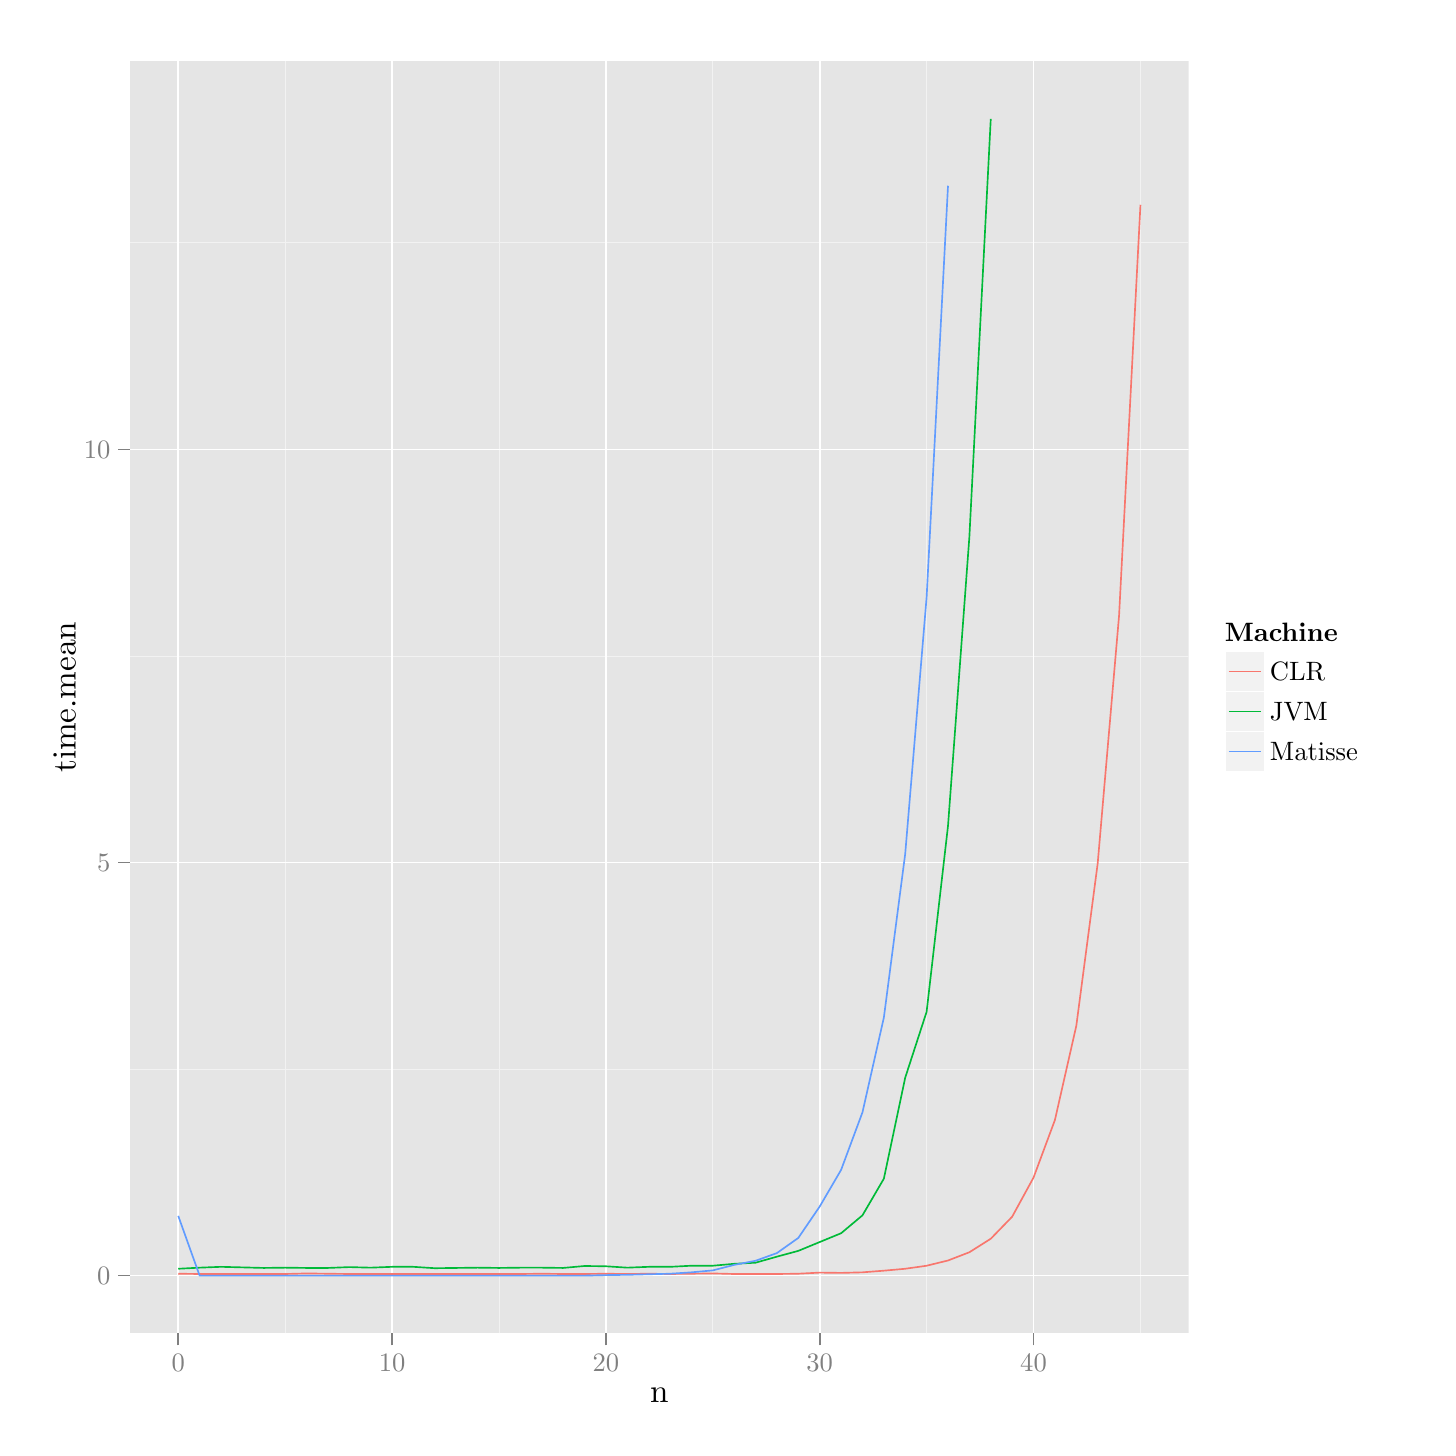
\begin{tikzpicture}[x=1pt,y=1pt]
\definecolor{fillColor}{RGB}{255,255,255}
\path[use as bounding box,fill=fillColor,fill opacity=0.00] (0,0) rectangle (505.89,505.89);
\begin{scope}
\path[clip] (  0.00,  0.00) rectangle (505.89,505.89);
\definecolor{drawColor}{RGB}{255,255,255}
\definecolor{fillColor}{RGB}{255,255,255}

\path[draw=drawColor,line width= 0.6pt,line join=round,line cap=round,fill=fillColor] (  0.00,  0.00) rectangle (505.89,505.89);
\end{scope}
\begin{scope}
\path[clip] ( 37.02, 34.03) rectangle (419.48,493.85);
\definecolor{fillColor}{gray}{0.90}

\path[fill=fillColor] ( 37.02, 34.03) rectangle (419.48,493.85);
\definecolor{drawColor}{gray}{0.95}

\path[draw=drawColor,line width= 0.3pt,line join=round] ( 37.02,129.58) --
	(419.48,129.58);

\path[draw=drawColor,line width= 0.3pt,line join=round] ( 37.02,278.87) --
	(419.48,278.87);

\path[draw=drawColor,line width= 0.3pt,line join=round] ( 37.02,428.16) --
	(419.48,428.16);

\path[draw=drawColor,line width= 0.3pt,line join=round] ( 93.04, 34.03) --
	( 93.04,493.85);

\path[draw=drawColor,line width= 0.3pt,line join=round] (170.30, 34.03) --
	(170.30,493.85);

\path[draw=drawColor,line width= 0.3pt,line join=round] (247.57, 34.03) --
	(247.57,493.85);

\path[draw=drawColor,line width= 0.3pt,line join=round] (324.83, 34.03) --
	(324.83,493.85);

\path[draw=drawColor,line width= 0.3pt,line join=round] (402.10, 34.03) --
	(402.10,493.85);
\definecolor{drawColor}{RGB}{255,255,255}

\path[draw=drawColor,line width= 0.6pt,line join=round] ( 37.02, 54.94) --
	(419.48, 54.94);

\path[draw=drawColor,line width= 0.6pt,line join=round] ( 37.02,204.22) --
	(419.48,204.22);

\path[draw=drawColor,line width= 0.6pt,line join=round] ( 37.02,353.51) --
	(419.48,353.51);

\path[draw=drawColor,line width= 0.6pt,line join=round] ( 54.41, 34.03) --
	( 54.41,493.85);

\path[draw=drawColor,line width= 0.6pt,line join=round] (131.67, 34.03) --
	(131.67,493.85);

\path[draw=drawColor,line width= 0.6pt,line join=round] (208.93, 34.03) --
	(208.93,493.85);

\path[draw=drawColor,line width= 0.6pt,line join=round] (286.20, 34.03) --
	(286.20,493.85);

\path[draw=drawColor,line width= 0.6pt,line join=round] (363.46, 34.03) --
	(363.46,493.85);
\definecolor{drawColor}{RGB}{248,118,109}

\path[draw=drawColor,line width= 0.6pt,line join=round] ( 54.41, 55.63) --
	( 62.13, 55.53) --
	( 69.86, 55.53) --
	( 77.58, 55.53) --
	( 85.31, 55.53) --
	( 93.04, 55.53) --
	(100.76, 55.73) --
	(108.49, 55.63) --
	(116.22, 55.53) --
	(123.94, 55.53) --
	(131.67, 55.53) --
	(139.40, 55.53) --
	(147.12, 55.53) --
	(154.85, 55.53) --
	(162.58, 55.53) --
	(170.30, 55.53) --
	(178.03, 55.53) --
	(185.75, 55.63) --
	(193.48, 55.53) --
	(201.21, 55.53) --
	(208.93, 55.63) --
	(216.66, 55.53) --
	(224.39, 55.63) --
	(232.11, 55.53) --
	(239.84, 55.63) --
	(247.57, 55.73) --
	(255.29, 55.53) --
	(263.02, 55.53) --
	(270.75, 55.53) --
	(278.47, 55.63) --
	(286.20, 56.03) --
	(293.93, 55.93) --
	(301.65, 56.13) --
	(309.38, 56.73) --
	(317.10, 57.42) --
	(324.83, 58.52) --
	(332.56, 60.41) --
	(340.28, 63.39) --
	(348.01, 68.27) --
	(355.74, 76.23) --
	(363.46, 90.37) --
	(371.19,111.17) --
	(378.92,145.21) --
	(386.64,203.83) --
	(394.37,293.40) --
	(402.10,441.89);
\definecolor{drawColor}{RGB}{0,186,56}

\path[draw=drawColor,line width= 0.6pt,line join=round] ( 54.41, 57.42) --
	( 62.13, 57.82) --
	( 69.86, 58.12) --
	( 77.58, 57.92) --
	( 85.31, 57.72) --
	( 93.04, 57.82) --
	(100.76, 57.72) --
	(108.49, 57.72) --
	(116.22, 58.02) --
	(123.94, 57.82) --
	(131.67, 58.12) --
	(139.40, 58.12) --
	(147.12, 57.62) --
	(154.85, 57.72) --
	(162.58, 57.82) --
	(170.30, 57.72) --
	(178.03, 57.82) --
	(185.75, 57.82) --
	(193.48, 57.72) --
	(201.21, 58.42) --
	(208.93, 58.32) --
	(216.66, 57.82) --
	(224.39, 58.12) --
	(232.11, 58.12) --
	(239.84, 58.52) --
	(247.57, 58.52) --
	(255.29, 59.21) --
	(263.02, 59.61) --
	(270.75, 61.80) --
	(278.47, 63.89) --
	(286.20, 67.08) --
	(293.93, 70.26) --
	(301.65, 76.73) --
	(309.38, 89.97) --
	(317.10,126.49) --
	(324.83,150.28) --
	(332.56,217.46) --
	(340.28,321.86) --
	(348.01,472.94);
\definecolor{drawColor}{RGB}{97,156,255}

\path[draw=drawColor,line width= 0.6pt,line join=round] ( 54.41, 76.53) --
	( 62.13, 54.94) --
	( 69.86, 54.94) --
	( 77.58, 54.94) --
	( 85.31, 54.94) --
	( 93.04, 54.94) --
	(100.76, 54.94) --
	(108.49, 54.94) --
	(116.22, 54.94) --
	(123.94, 54.94) --
	(131.67, 54.94) --
	(139.40, 54.94) --
	(147.12, 54.94) --
	(154.85, 54.94) --
	(162.58, 54.94) --
	(170.30, 54.94) --
	(178.03, 54.94) --
	(185.75, 54.94) --
	(193.48, 54.94) --
	(201.21, 54.94) --
	(208.93, 55.13) --
	(216.66, 55.23) --
	(224.39, 55.43) --
	(232.11, 55.63) --
	(239.84, 56.13) --
	(247.57, 56.83) --
	(255.29, 58.82) --
	(263.02, 60.31) --
	(270.75, 63.10) --
	(278.47, 68.57) --
	(286.20, 79.92) --
	(293.93, 93.15) --
	(301.65,113.95) --
	(309.38,148.19) --
	(317.10,207.41) --
	(324.83,300.07) --
	(332.56,448.76);
\end{scope}
\begin{scope}
\path[clip] (  0.00,  0.00) rectangle (505.89,505.89);
\definecolor{drawColor}{gray}{0.50}

\node[text=drawColor,anchor=base east,inner sep=0pt, outer sep=0pt, scale=  0.96] at ( 29.91, 51.63) {0};

\node[text=drawColor,anchor=base east,inner sep=0pt, outer sep=0pt, scale=  0.96] at ( 29.91,200.92) {5};

\node[text=drawColor,anchor=base east,inner sep=0pt, outer sep=0pt, scale=  0.96] at ( 29.91,350.21) {10};
\end{scope}
\begin{scope}
\path[clip] (  0.00,  0.00) rectangle (505.89,505.89);
\definecolor{drawColor}{gray}{0.50}

\path[draw=drawColor,line width= 0.6pt,line join=round] ( 32.75, 54.94) --
	( 37.02, 54.94);

\path[draw=drawColor,line width= 0.6pt,line join=round] ( 32.75,204.22) --
	( 37.02,204.22);

\path[draw=drawColor,line width= 0.6pt,line join=round] ( 32.75,353.51) --
	( 37.02,353.51);
\end{scope}
\begin{scope}
\path[clip] (  0.00,  0.00) rectangle (505.89,505.89);
\definecolor{drawColor}{gray}{0.50}

\path[draw=drawColor,line width= 0.6pt,line join=round] ( 54.41, 29.77) --
	( 54.41, 34.03);

\path[draw=drawColor,line width= 0.6pt,line join=round] (131.67, 29.77) --
	(131.67, 34.03);

\path[draw=drawColor,line width= 0.6pt,line join=round] (208.93, 29.77) --
	(208.93, 34.03);

\path[draw=drawColor,line width= 0.6pt,line join=round] (286.20, 29.77) --
	(286.20, 34.03);

\path[draw=drawColor,line width= 0.6pt,line join=round] (363.46, 29.77) --
	(363.46, 34.03);
\end{scope}
\begin{scope}
\path[clip] (  0.00,  0.00) rectangle (505.89,505.89);
\definecolor{drawColor}{gray}{0.50}

\node[text=drawColor,anchor=base,inner sep=0pt, outer sep=0pt, scale=  0.96] at ( 54.41, 20.31) {0};

\node[text=drawColor,anchor=base,inner sep=0pt, outer sep=0pt, scale=  0.96] at (131.67, 20.31) {10};

\node[text=drawColor,anchor=base,inner sep=0pt, outer sep=0pt, scale=  0.96] at (208.93, 20.31) {20};

\node[text=drawColor,anchor=base,inner sep=0pt, outer sep=0pt, scale=  0.96] at (286.20, 20.31) {30};

\node[text=drawColor,anchor=base,inner sep=0pt, outer sep=0pt, scale=  0.96] at (363.46, 20.31) {40};
\end{scope}
\begin{scope}
\path[clip] (  0.00,  0.00) rectangle (505.89,505.89);
\definecolor{drawColor}{RGB}{0,0,0}

\node[text=drawColor,anchor=base,inner sep=0pt, outer sep=0pt, scale=  1.20] at (228.25,  9.03) {n};
\end{scope}
\begin{scope}
\path[clip] (  0.00,  0.00) rectangle (505.89,505.89);
\definecolor{drawColor}{RGB}{0,0,0}

\node[text=drawColor,rotate= 90.00,anchor=base,inner sep=0pt, outer sep=0pt, scale=  1.20] at ( 17.30,263.94) {time.mean};
\end{scope}
\begin{scope}
\path[clip] (  0.00,  0.00) rectangle (505.89,505.89);
\definecolor{fillColor}{RGB}{255,255,255}

\path[fill=fillColor] (428.35,232.87) rectangle (484.98,295.01);
\end{scope}
\begin{scope}
\path[clip] (  0.00,  0.00) rectangle (505.89,505.89);
\definecolor{drawColor}{RGB}{0,0,0}

\node[text=drawColor,anchor=base west,inner sep=0pt, outer sep=0pt, scale=  0.96] at (432.62,284.11) {\bfseries Machine};
\end{scope}
\begin{scope}
\path[clip] (  0.00,  0.00) rectangle (505.89,505.89);
\definecolor{drawColor}{RGB}{255,255,255}
\definecolor{fillColor}{gray}{0.95}

\path[draw=drawColor,line width= 0.6pt,line join=round,line cap=round,fill=fillColor] (432.62,266.05) rectangle (447.07,280.50);
\end{scope}
\begin{scope}
\path[clip] (  0.00,  0.00) rectangle (505.89,505.89);
\definecolor{drawColor}{RGB}{248,118,109}

\path[draw=drawColor,line width= 0.6pt,line join=round] (434.06,273.27) -- (445.62,273.27);
\end{scope}
\begin{scope}
\path[clip] (  0.00,  0.00) rectangle (505.89,505.89);
\definecolor{drawColor}{RGB}{255,255,255}
\definecolor{fillColor}{gray}{0.95}

\path[draw=drawColor,line width= 0.6pt,line join=round,line cap=round,fill=fillColor] (432.62,251.59) rectangle (447.07,266.05);
\end{scope}
\begin{scope}
\path[clip] (  0.00,  0.00) rectangle (505.89,505.89);
\definecolor{drawColor}{RGB}{0,186,56}

\path[draw=drawColor,line width= 0.6pt,line join=round] (434.06,258.82) -- (445.62,258.82);
\end{scope}
\begin{scope}
\path[clip] (  0.00,  0.00) rectangle (505.89,505.89);
\definecolor{drawColor}{RGB}{255,255,255}
\definecolor{fillColor}{gray}{0.95}

\path[draw=drawColor,line width= 0.6pt,line join=round,line cap=round,fill=fillColor] (432.62,237.14) rectangle (447.07,251.59);
\end{scope}
\begin{scope}
\path[clip] (  0.00,  0.00) rectangle (505.89,505.89);
\definecolor{drawColor}{RGB}{97,156,255}

\path[draw=drawColor,line width= 0.6pt,line join=round] (434.06,244.37) -- (445.62,244.37);
\end{scope}
\begin{scope}
\path[clip] (  0.00,  0.00) rectangle (505.89,505.89);
\definecolor{drawColor}{RGB}{0,0,0}

\node[text=drawColor,anchor=base west,inner sep=0pt, outer sep=0pt, scale=  0.96] at (448.88,269.97) {CLR};
\end{scope}
\begin{scope}
\path[clip] (  0.00,  0.00) rectangle (505.89,505.89);
\definecolor{drawColor}{RGB}{0,0,0}

\node[text=drawColor,anchor=base west,inner sep=0pt, outer sep=0pt, scale=  0.96] at (448.88,255.51) {JVM};
\end{scope}
\begin{scope}
\path[clip] (  0.00,  0.00) rectangle (505.89,505.89);
\definecolor{drawColor}{RGB}{0,0,0}

\node[text=drawColor,anchor=base west,inner sep=0pt, outer sep=0pt, scale=  0.96] at (448.88,241.06) {Matisse};
\end{scope}
\end{tikzpicture}
}
  \caption{Mean running time of $fib(n)$}
\label{fig:eval:benchmark:fib}
\end{figure}

The graph shows the $fib(n)$ on x-axis and mean time on the y-axis. \thename{}
is almost on par with JVM, both of which lack behind CLR. That is an indication
of efficient sub-routine and stack memory mechanisms in \thename{}. It is
important to remember that these are all na\"ive implementations with no
optimizations such as tail-recursion or dynamic programming techniques, which
would have a significant impact on the running time.

% invocation

The sub-routing benchmark is implemented in a similar fashion as the stack
workout program, only the calculation is performed in a sub-routine which is
invoked each iteration. All the stack operations done in the sub-routine are
executed in constant time, which given the resulting running time of
$T(n) = O(n) \cdot O(k) = O(n)$, where $k$ is the constant number of stack
operations. For invoking the sub-routine we use the \instr{invoke} instructions,
while CLR uses {\tt call} and JVM uses {\tt invokestatic}. The result of the
benchmark can be seen below, in Figure~\ref{fig:eval:benchmark:invoc}.

\begin{figure}[H]
  \centering
  \scalebox{0.8}[0.6]{% Created by tikzDevice version 0.8.1 on 2015-06-28 01:47:35
% !TEX encoding = UTF-8 Unicode
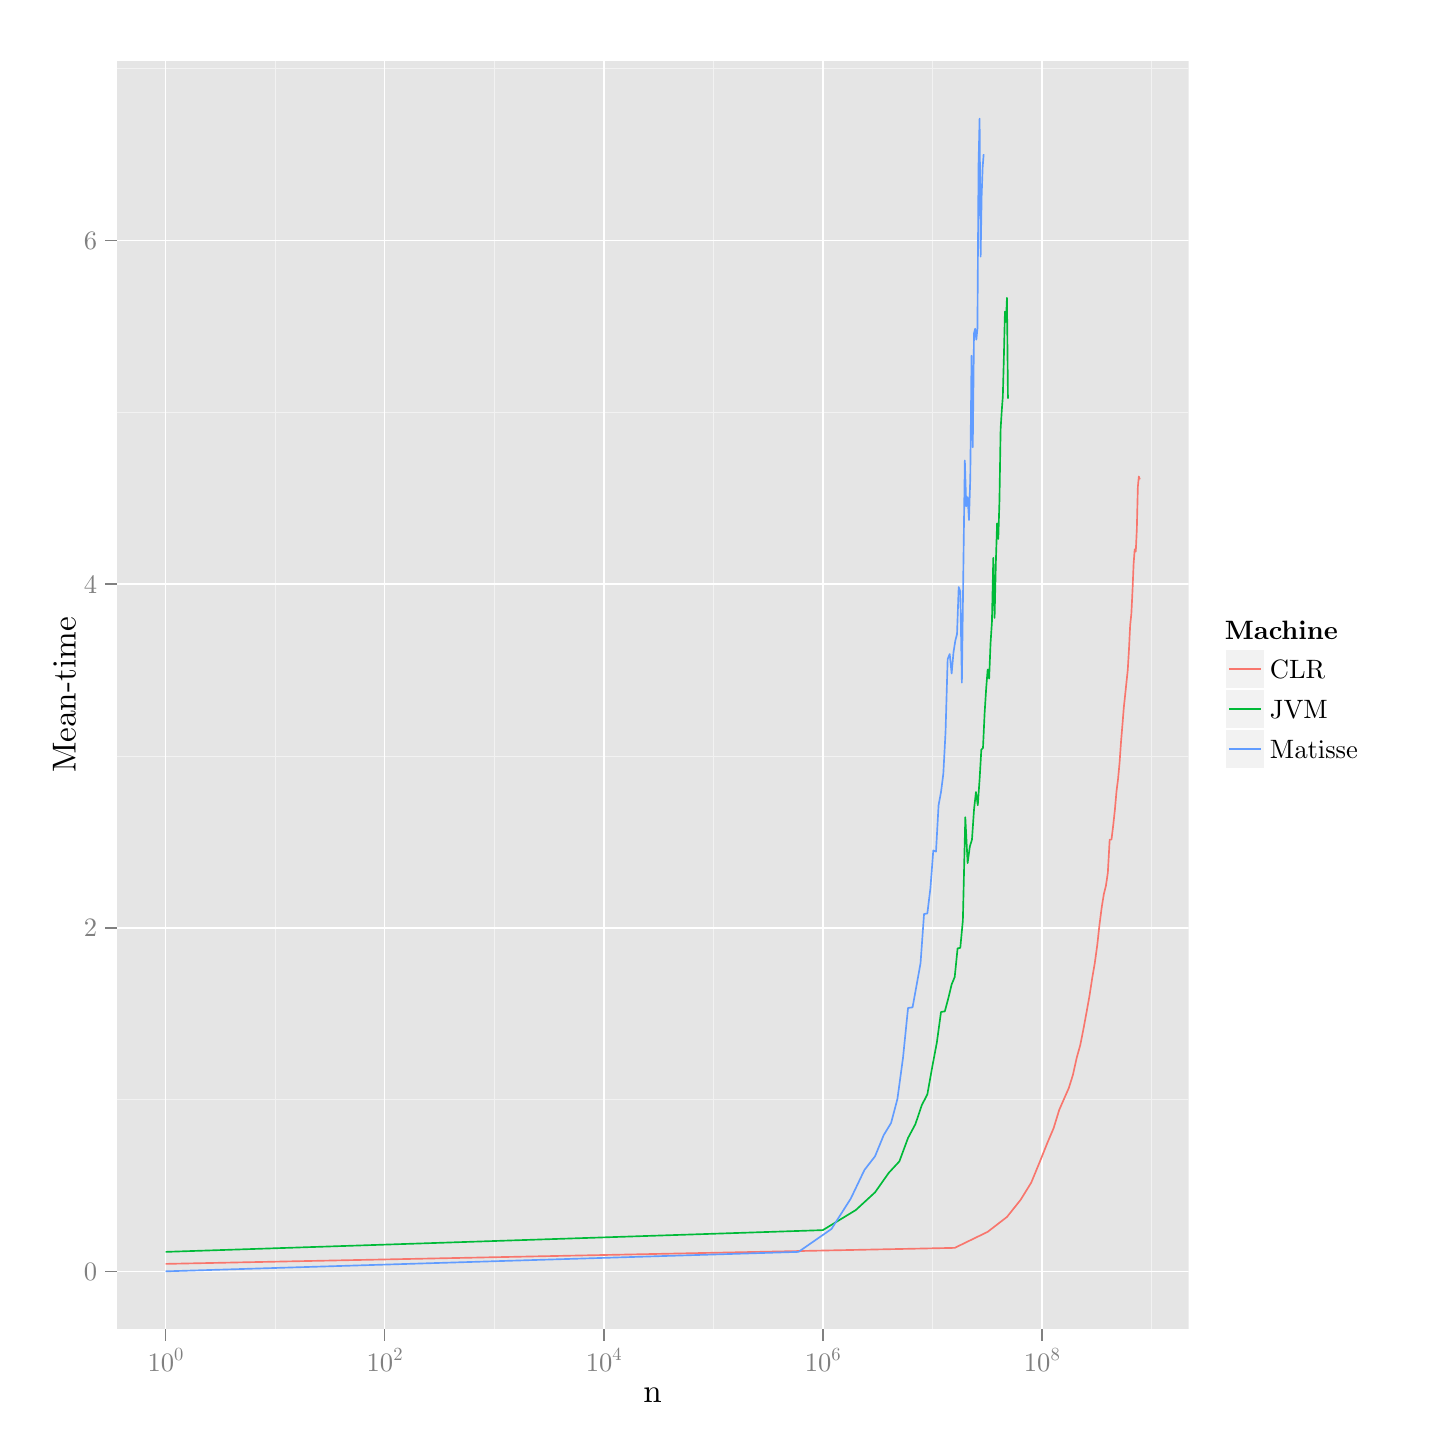
\begin{tikzpicture}[x=1pt,y=1pt]
\definecolor{fillColor}{RGB}{255,255,255}
\path[use as bounding box,fill=fillColor,fill opacity=0.00] (0,0) rectangle (505.89,505.89);
\begin{scope}
\path[clip] (  0.00,  0.00) rectangle (505.89,505.89);
\definecolor{drawColor}{RGB}{255,255,255}
\definecolor{fillColor}{RGB}{255,255,255}

\path[draw=drawColor,line width= 0.6pt,line join=round,line cap=round,fill=fillColor] (  0.00,  0.00) rectangle (505.89,505.89);
\end{scope}
\begin{scope}
\path[clip] ( 32.22, 35.66) rectangle (419.48,493.85);
\definecolor{fillColor}{gray}{0.90}

\path[fill=fillColor] ( 32.22, 35.66) rectangle (419.48,493.85);
\definecolor{drawColor}{gray}{0.95}

\path[draw=drawColor,line width= 0.3pt,line join=round] ( 32.22,118.56) --
	(419.48,118.56);

\path[draw=drawColor,line width= 0.3pt,line join=round] ( 32.22,242.72) --
	(419.48,242.72);

\path[draw=drawColor,line width= 0.3pt,line join=round] ( 32.22,366.87) --
	(419.48,366.87);

\path[draw=drawColor,line width= 0.3pt,line join=round] ( 32.22,491.02) --
	(419.48,491.02);

\path[draw=drawColor,line width= 0.3pt,line join=round] ( 89.41, 35.66) --
	( 89.41,493.85);

\path[draw=drawColor,line width= 0.3pt,line join=round] (168.57, 35.66) --
	(168.57,493.85);

\path[draw=drawColor,line width= 0.3pt,line join=round] (247.73, 35.66) --
	(247.73,493.85);

\path[draw=drawColor,line width= 0.3pt,line join=round] (326.90, 35.66) --
	(326.90,493.85);

\path[draw=drawColor,line width= 0.3pt,line join=round] (406.06, 35.66) --
	(406.06,493.85);
\definecolor{drawColor}{RGB}{255,255,255}

\path[draw=drawColor,line width= 0.6pt,line join=round] ( 32.22, 56.49) --
	(419.48, 56.49);

\path[draw=drawColor,line width= 0.6pt,line join=round] ( 32.22,180.64) --
	(419.48,180.64);

\path[draw=drawColor,line width= 0.6pt,line join=round] ( 32.22,304.79) --
	(419.48,304.79);

\path[draw=drawColor,line width= 0.6pt,line join=round] ( 32.22,428.94) --
	(419.48,428.94);

\path[draw=drawColor,line width= 0.6pt,line join=round] ( 49.82, 35.66) --
	( 49.82,493.85);

\path[draw=drawColor,line width= 0.6pt,line join=round] (128.99, 35.66) --
	(128.99,493.85);

\path[draw=drawColor,line width= 0.6pt,line join=round] (208.15, 35.66) --
	(208.15,493.85);

\path[draw=drawColor,line width= 0.6pt,line join=round] (287.32, 35.66) --
	(287.32,493.85);

\path[draw=drawColor,line width= 0.6pt,line join=round] (366.48, 35.66) --
	(366.48,493.85);
\definecolor{drawColor}{RGB}{248,118,109}

\path[draw=drawColor,line width= 0.6pt,line join=round] ( 49.82, 59.18) --
	(334.98, 64.97) --
	(346.89, 70.76) --
	(353.86, 76.14) --
	(358.81, 82.35) --
	(362.64, 88.56) --
	(365.78, 96.21) --
	(368.43,102.84) --
	(370.72,108.22) --
	(372.75,114.84) --
	(374.56,118.98) --
	(376.20,122.70) --
	(377.69,127.46) --
	(379.07,133.67) --
	(380.34,138.22) --
	(381.53,144.22) --
	(382.64,150.22) --
	(383.68,156.02) --
	(384.66,162.43) --
	(385.59,167.81) --
	(386.47,174.22) --
	(387.31,181.88) --
	(388.11,188.09) --
	(388.88,192.85) --
	(389.61,195.74) --
	(390.31,200.50) --
	(390.98,212.50) --
	(391.63,212.50) --
	(392.26,217.68) --
	(392.86,223.26) --
	(393.44,229.89) --
	(394.01,234.44) --
	(394.55,240.23) --
	(395.08,247.89) --
	(395.60,254.10) --
	(396.09,260.30) --
	(396.58,264.86) --
	(397.05,269.41) --
	(397.51,273.75) --
	(397.95,281.20) --
	(398.39,290.10) --
	(398.81,294.03) --
	(399.23,302.52) --
	(399.63,312.24) --
	(400.03,317.41) --
	(400.41,316.59) --
	(400.79,324.66) --
	(401.16,339.97) --
	(401.52,343.69) --
	(401.88,342.66);
\definecolor{drawColor}{RGB}{0,186,56}

\path[draw=drawColor,line width= 0.6pt,line join=round] ( 49.82, 63.52) --
	(287.32, 71.38) --
	(299.23, 78.63) --
	(306.20, 85.04) --
	(311.15, 92.08) --
	(314.98, 96.21) --
	(318.12,104.70) --
	(320.77,109.66) --
	(323.06,116.49) --
	(325.09,120.42) --
	(326.90,130.56) --
	(328.54,139.25) --
	(330.03,150.22) --
	(331.41,150.43) --
	(332.68,155.19) --
	(333.87,160.15) --
	(334.98,162.84) --
	(336.02,173.19) --
	(337.00,173.40) --
	(337.93,183.33) --
	(338.81,220.57) --
	(339.65,204.02) --
	(340.45,210.02) --
	(341.22,212.50) --
	(341.95,223.26) --
	(342.65,229.68) --
	(343.32,224.92) --
	(343.97,234.23) --
	(344.60,244.99) --
	(345.20,245.61) --
	(345.78,258.03) --
	(346.35,267.13) --
	(346.89,273.96) --
	(347.42,270.65) --
	(347.93,283.48) --
	(348.43,291.13) --
	(348.92,314.31) --
	(349.39,292.58) --
	(349.85,312.65) --
	(350.29,326.73) --
	(350.73,321.14) --
	(351.15,335.00) --
	(351.57,360.87) --
	(351.97,367.28) --
	(352.37,372.66) --
	(352.75,386.94) --
	(353.13,403.29) --
	(353.50,399.56) --
	(353.86,408.25) --
	(354.22,371.83);
\definecolor{drawColor}{RGB}{97,156,255}

\path[draw=drawColor,line width= 0.6pt,line join=round] ( 49.82, 56.49) --
	(278.53, 63.52) --
	(290.45, 71.80) --
	(297.42, 82.77) --
	(302.36, 93.11) --
	(306.20, 98.08) --
	(309.33,105.73) --
	(311.98,110.08) --
	(314.28,118.77) --
	(316.30,133.67) --
	(318.12,151.67) --
	(319.75,151.88) --
	(321.25,160.15) --
	(322.63,167.81) --
	(323.90,185.60) --
	(325.09,185.81) --
	(326.20,194.92) --
	(327.24,208.57) --
	(328.22,208.16) --
	(329.15,224.92) --
	(330.03,229.68) --
	(330.87,236.30) --
	(331.67,251.41) --
	(332.43,277.68) --
	(333.17,279.55) --
	(333.87,272.51) --
	(334.54,280.17) --
	(335.19,284.31) --
	(335.82,286.79) --
	(336.42,303.76) --
	(337.00,302.10) --
	(337.57,269.20) --
	(338.11,310.79) --
	(338.64,349.49) --
	(339.15,332.93) --
	(339.65,336.24) --
	(340.14,327.97) --
	(340.61,343.28) --
	(341.06,387.35) --
	(341.51,354.25) --
	(341.95,395.42) --
	(342.37,397.08) --
	(342.79,393.15) --
	(343.19,397.08) --
	(343.59,456.46) --
	(343.97,473.02) --
	(344.35,423.15) --
	(344.72,445.29) --
	(345.08,455.43) --
	(345.44,460.19);
\end{scope}
\begin{scope}
\path[clip] (  0.00,  0.00) rectangle (505.89,505.89);
\definecolor{drawColor}{gray}{0.50}

\node[text=drawColor,anchor=base east,inner sep=0pt, outer sep=0pt, scale=  0.96] at ( 25.11, 53.18) {0};

\node[text=drawColor,anchor=base east,inner sep=0pt, outer sep=0pt, scale=  0.96] at ( 25.11,177.33) {2};

\node[text=drawColor,anchor=base east,inner sep=0pt, outer sep=0pt, scale=  0.96] at ( 25.11,301.49) {4};

\node[text=drawColor,anchor=base east,inner sep=0pt, outer sep=0pt, scale=  0.96] at ( 25.11,425.64) {6};
\end{scope}
\begin{scope}
\path[clip] (  0.00,  0.00) rectangle (505.89,505.89);
\definecolor{drawColor}{gray}{0.50}

\path[draw=drawColor,line width= 0.6pt,line join=round] ( 27.95, 56.49) --
	( 32.22, 56.49);

\path[draw=drawColor,line width= 0.6pt,line join=round] ( 27.95,180.64) --
	( 32.22,180.64);

\path[draw=drawColor,line width= 0.6pt,line join=round] ( 27.95,304.79) --
	( 32.22,304.79);

\path[draw=drawColor,line width= 0.6pt,line join=round] ( 27.95,428.94) --
	( 32.22,428.94);
\end{scope}
\begin{scope}
\path[clip] (  0.00,  0.00) rectangle (505.89,505.89);
\definecolor{drawColor}{gray}{0.50}

\path[draw=drawColor,line width= 0.6pt,line join=round] ( 49.82, 31.39) --
	( 49.82, 35.66);

\path[draw=drawColor,line width= 0.6pt,line join=round] (128.99, 31.39) --
	(128.99, 35.66);

\path[draw=drawColor,line width= 0.6pt,line join=round] (208.15, 31.39) --
	(208.15, 35.66);

\path[draw=drawColor,line width= 0.6pt,line join=round] (287.32, 31.39) --
	(287.32, 35.66);

\path[draw=drawColor,line width= 0.6pt,line join=round] (366.48, 31.39) --
	(366.48, 35.66);
\end{scope}
\begin{scope}
\path[clip] (  0.00,  0.00) rectangle (505.89,505.89);
\definecolor{drawColor}{gray}{0.50}

\node[text=drawColor,anchor=base west,inner sep=0pt, outer sep=0pt, scale=  0.96] at ( 43.35, 20.31) {10};

\node[text=drawColor,anchor=base west,inner sep=0pt, outer sep=0pt, scale=  0.67] at ( 52.94, 24.24) {0};

\node[text=drawColor,anchor=base west,inner sep=0pt, outer sep=0pt, scale=  0.96] at (122.51, 20.31) {10};

\node[text=drawColor,anchor=base west,inner sep=0pt, outer sep=0pt, scale=  0.67] at (132.11, 24.24) {2};

\node[text=drawColor,anchor=base west,inner sep=0pt, outer sep=0pt, scale=  0.96] at (201.67, 20.31) {10};

\node[text=drawColor,anchor=base west,inner sep=0pt, outer sep=0pt, scale=  0.67] at (211.27, 24.24) {4};

\node[text=drawColor,anchor=base west,inner sep=0pt, outer sep=0pt, scale=  0.96] at (280.84, 20.31) {10};

\node[text=drawColor,anchor=base west,inner sep=0pt, outer sep=0pt, scale=  0.67] at (290.43, 24.24) {6};

\node[text=drawColor,anchor=base west,inner sep=0pt, outer sep=0pt, scale=  0.96] at (360.00, 20.31) {10};

\node[text=drawColor,anchor=base west,inner sep=0pt, outer sep=0pt, scale=  0.67] at (369.60, 24.24) {8};
\end{scope}
\begin{scope}
\path[clip] (  0.00,  0.00) rectangle (505.89,505.89);
\definecolor{drawColor}{RGB}{0,0,0}

\node[text=drawColor,anchor=base,inner sep=0pt, outer sep=0pt, scale=  1.20] at (225.85,  9.03) {n};
\end{scope}
\begin{scope}
\path[clip] (  0.00,  0.00) rectangle (505.89,505.89);
\definecolor{drawColor}{RGB}{0,0,0}

\node[text=drawColor,rotate= 90.00,anchor=base,inner sep=0pt, outer sep=0pt, scale=  1.20] at ( 17.30,264.75) {Mean-time};
\end{scope}
\begin{scope}
\path[clip] (  0.00,  0.00) rectangle (505.89,505.89);
\definecolor{fillColor}{RGB}{255,255,255}

\path[fill=fillColor] (428.35,233.68) rectangle (484.98,295.82);
\end{scope}
\begin{scope}
\path[clip] (  0.00,  0.00) rectangle (505.89,505.89);
\definecolor{drawColor}{RGB}{0,0,0}

\node[text=drawColor,anchor=base west,inner sep=0pt, outer sep=0pt, scale=  0.96] at (432.62,284.93) {\bfseries Machine};
\end{scope}
\begin{scope}
\path[clip] (  0.00,  0.00) rectangle (505.89,505.89);
\definecolor{drawColor}{RGB}{255,255,255}
\definecolor{fillColor}{gray}{0.95}

\path[draw=drawColor,line width= 0.6pt,line join=round,line cap=round,fill=fillColor] (432.62,266.86) rectangle (447.07,281.31);
\end{scope}
\begin{scope}
\path[clip] (  0.00,  0.00) rectangle (505.89,505.89);
\definecolor{drawColor}{RGB}{248,118,109}

\path[draw=drawColor,line width= 0.6pt,line join=round] (434.06,274.09) -- (445.62,274.09);
\end{scope}
\begin{scope}
\path[clip] (  0.00,  0.00) rectangle (505.89,505.89);
\definecolor{drawColor}{RGB}{255,255,255}
\definecolor{fillColor}{gray}{0.95}

\path[draw=drawColor,line width= 0.6pt,line join=round,line cap=round,fill=fillColor] (432.62,252.41) rectangle (447.07,266.86);
\end{scope}
\begin{scope}
\path[clip] (  0.00,  0.00) rectangle (505.89,505.89);
\definecolor{drawColor}{RGB}{0,186,56}

\path[draw=drawColor,line width= 0.6pt,line join=round] (434.06,259.63) -- (445.62,259.63);
\end{scope}
\begin{scope}
\path[clip] (  0.00,  0.00) rectangle (505.89,505.89);
\definecolor{drawColor}{RGB}{255,255,255}
\definecolor{fillColor}{gray}{0.95}

\path[draw=drawColor,line width= 0.6pt,line join=round,line cap=round,fill=fillColor] (432.62,237.95) rectangle (447.07,252.41);
\end{scope}
\begin{scope}
\path[clip] (  0.00,  0.00) rectangle (505.89,505.89);
\definecolor{drawColor}{RGB}{97,156,255}

\path[draw=drawColor,line width= 0.6pt,line join=round] (434.06,245.18) -- (445.62,245.18);
\end{scope}
\begin{scope}
\path[clip] (  0.00,  0.00) rectangle (505.89,505.89);
\definecolor{drawColor}{RGB}{0,0,0}

\node[text=drawColor,anchor=base west,inner sep=0pt, outer sep=0pt, scale=  0.96] at (448.88,270.78) {CLR};
\end{scope}
\begin{scope}
\path[clip] (  0.00,  0.00) rectangle (505.89,505.89);
\definecolor{drawColor}{RGB}{0,0,0}

\node[text=drawColor,anchor=base west,inner sep=0pt, outer sep=0pt, scale=  0.96] at (448.88,256.33) {JVM};
\end{scope}
\begin{scope}
\path[clip] (  0.00,  0.00) rectangle (505.89,505.89);
\definecolor{drawColor}{RGB}{0,0,0}

\node[text=drawColor,anchor=base west,inner sep=0pt, outer sep=0pt, scale=  0.96] at (448.88,241.87) {Matisse};
\end{scope}
\end{tikzpicture}
}
  \caption{Mean running time of sub-routine workout}
\label{fig:eval:benchmark:invoc}
\end{figure}

Again \thename{} is \emph{relatively} close to JVM. It is interesting that the
graph for both JVM and \thename{} is jagged for high values of $n$ while CLRs
performance shows a more steady curve. Exactly what this is due to is difficult
to say.

% heap objects

The last benchmark focuses on field operations on heap objects, namely the
\instr{pushFieldHeapObject} and \instr{popFieldHeapObject} instructions. It does
this by initially creating an instance of a simple heap object with a single
integer field. It then does $n$ iterations of pushing it's field onto the stack,
incrementing it and popping it back to the heap object. The running time becomes
the same as the sub-routine benchmark; $T(n) = O(n) \cdot O(k) = O(n)$, where
$k$ is the constant number of stack operations. The result of the benchmark can
be seen below, in Figure~\ref{fig:eval:benchmark:heap}.

\begin{figure}[H]
  \centering
  \scalebox{0.8}[0.6]{% Created by tikzDevice version 0.8.1 on 2015-06-28 20:20:30
% !TEX encoding = UTF-8 Unicode
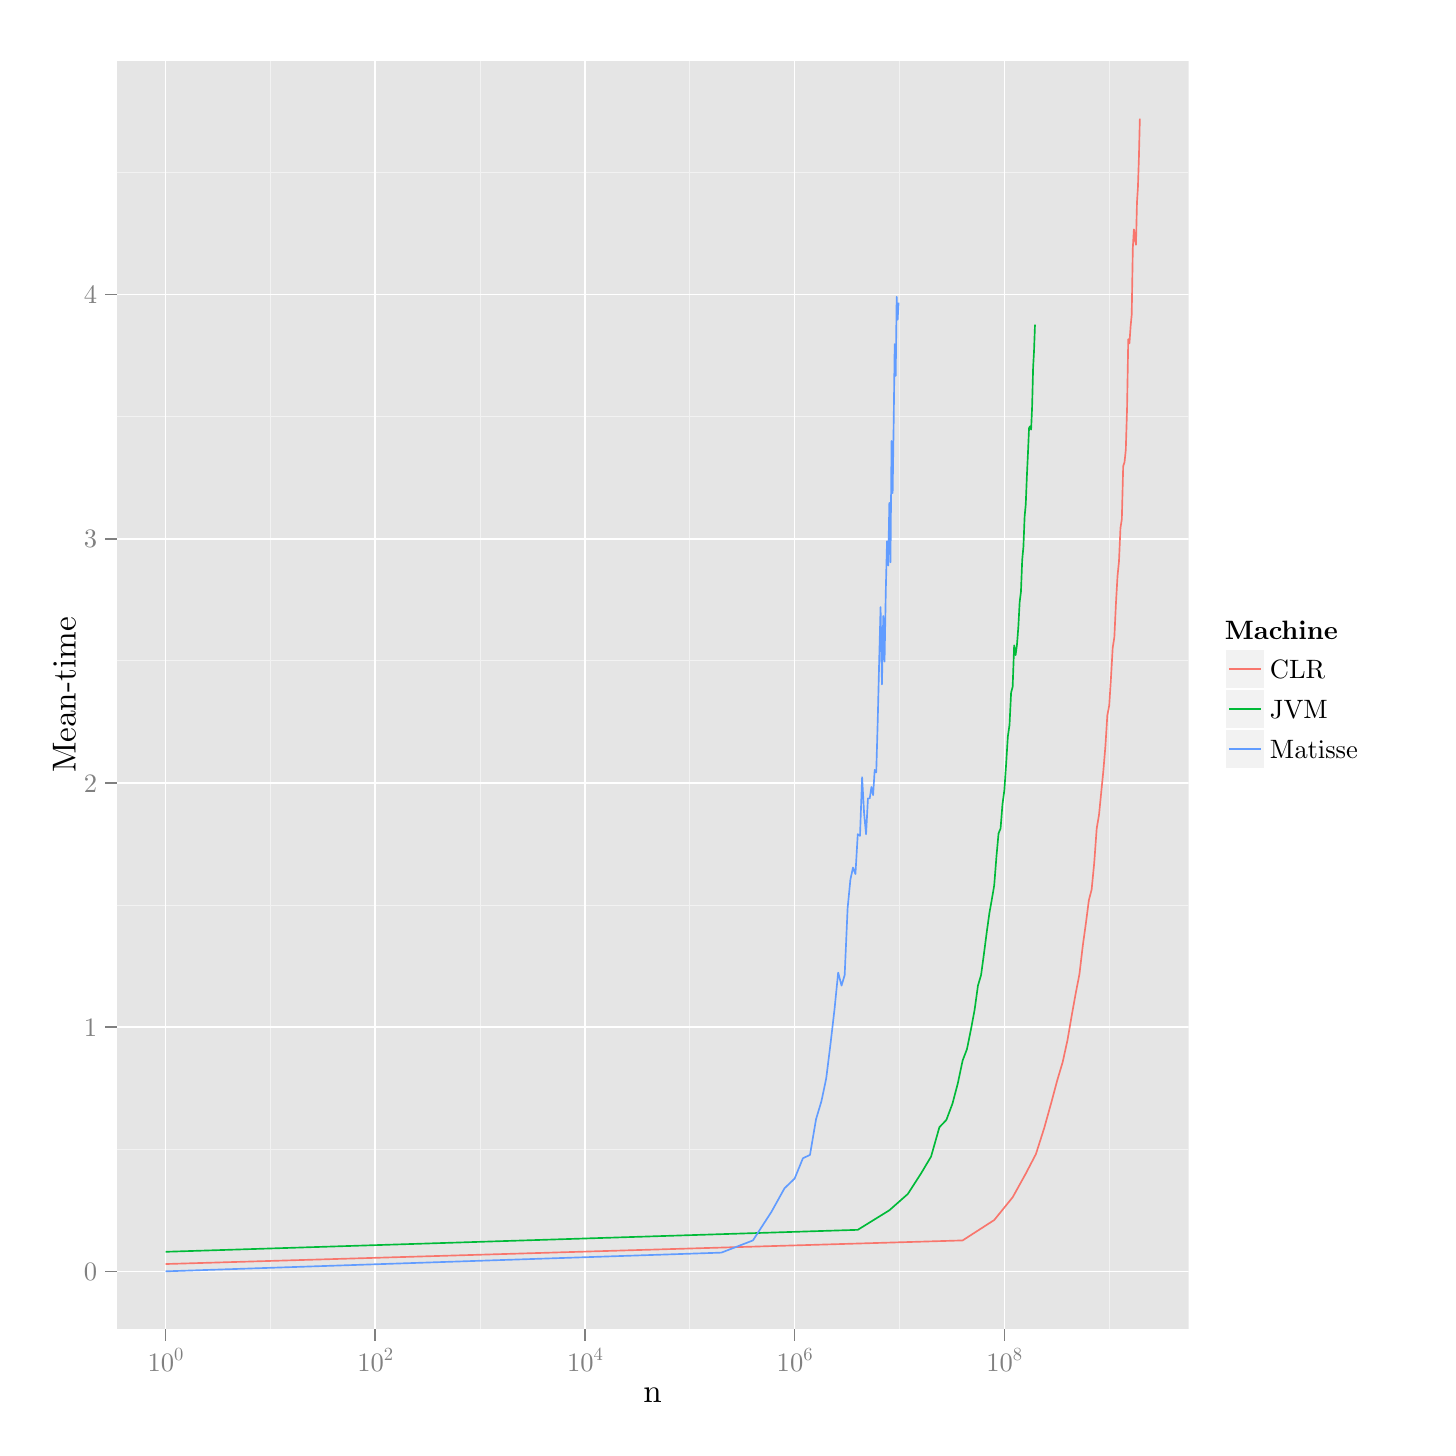
\begin{tikzpicture}[x=1pt,y=1pt]
\definecolor{fillColor}{RGB}{255,255,255}
\path[use as bounding box,fill=fillColor,fill opacity=0.00] (0,0) rectangle (505.89,505.89);
\begin{scope}
\path[clip] (  0.00,  0.00) rectangle (505.89,505.89);
\definecolor{drawColor}{RGB}{255,255,255}
\definecolor{fillColor}{RGB}{255,255,255}

\path[draw=drawColor,line width= 0.6pt,line join=round,line cap=round,fill=fillColor] (  0.00,  0.00) rectangle (505.89,505.89);
\end{scope}
\begin{scope}
\path[clip] ( 32.22, 35.66) rectangle (419.48,493.85);
\definecolor{fillColor}{gray}{0.90}

\path[fill=fillColor] ( 32.22, 35.66) rectangle (419.48,493.85);
\definecolor{drawColor}{gray}{0.95}

\path[draw=drawColor,line width= 0.3pt,line join=round] ( 32.22,100.61) --
	(419.48,100.61);

\path[draw=drawColor,line width= 0.3pt,line join=round] ( 32.22,188.86) --
	(419.48,188.86);

\path[draw=drawColor,line width= 0.3pt,line join=round] ( 32.22,277.11) --
	(419.48,277.11);

\path[draw=drawColor,line width= 0.3pt,line join=round] ( 32.22,365.36) --
	(419.48,365.36);

\path[draw=drawColor,line width= 0.3pt,line join=round] ( 32.22,453.60) --
	(419.48,453.60);

\path[draw=drawColor,line width= 0.3pt,line join=round] ( 87.71, 35.66) --
	( 87.71,493.85);

\path[draw=drawColor,line width= 0.3pt,line join=round] (163.48, 35.66) --
	(163.48,493.85);

\path[draw=drawColor,line width= 0.3pt,line join=round] (239.26, 35.66) --
	(239.26,493.85);

\path[draw=drawColor,line width= 0.3pt,line join=round] (315.03, 35.66) --
	(315.03,493.85);

\path[draw=drawColor,line width= 0.3pt,line join=round] (390.81, 35.66) --
	(390.81,493.85);
\definecolor{drawColor}{RGB}{255,255,255}

\path[draw=drawColor,line width= 0.6pt,line join=round] ( 32.22, 56.49) --
	(419.48, 56.49);

\path[draw=drawColor,line width= 0.6pt,line join=round] ( 32.22,144.73) --
	(419.48,144.73);

\path[draw=drawColor,line width= 0.6pt,line join=round] ( 32.22,232.98) --
	(419.48,232.98);

\path[draw=drawColor,line width= 0.6pt,line join=round] ( 32.22,321.23) --
	(419.48,321.23);

\path[draw=drawColor,line width= 0.6pt,line join=round] ( 32.22,409.48) --
	(419.48,409.48);

\path[draw=drawColor,line width= 0.6pt,line join=round] ( 49.82, 35.66) --
	( 49.82,493.85);

\path[draw=drawColor,line width= 0.6pt,line join=round] (125.60, 35.66) --
	(125.60,493.85);

\path[draw=drawColor,line width= 0.6pt,line join=round] (201.37, 35.66) --
	(201.37,493.85);

\path[draw=drawColor,line width= 0.6pt,line join=round] (277.14, 35.66) --
	(277.14,493.85);

\path[draw=drawColor,line width= 0.6pt,line join=round] (352.92, 35.66) --
	(352.92,493.85);
\definecolor{drawColor}{RGB}{248,118,109}

\path[draw=drawColor,line width= 0.6pt,line join=round] ( 49.82, 59.13) --
	(337.84, 67.66) --
	(349.25, 75.02) --
	(355.92, 83.25) --
	(360.65, 91.79) --
	(364.32, 98.85) --
	(367.32,108.26) --
	(369.86,117.38) --
	(372.06,125.61) --
	(373.99,132.09) --
	(375.73,140.03) --
	(377.30,149.15) --
	(378.73,157.09) --
	(380.05,163.85) --
	(381.26,174.15) --
	(382.40,182.39) --
	(383.46,190.62) --
	(384.46,194.45) --
	(385.40,204.16) --
	(386.29,216.51) --
	(387.13,221.51) --
	(387.94,229.75) --
	(388.70,237.40) --
	(389.43,246.22) --
	(390.13,257.40) --
	(390.81,260.93) --
	(391.45,270.93) --
	(392.07,281.81) --
	(392.67,285.64) --
	(393.25,297.99) --
	(393.81,307.70) --
	(394.34,312.99) --
	(394.87,325.06) --
	(395.37,328.29) --
	(395.86,347.41) --
	(396.34,348.88) --
	(396.80,353.29) --
	(397.26,368.30) --
	(397.69,393.30) --
	(398.12,391.83) --
	(398.54,398.01) --
	(398.94,402.13) --
	(399.34,426.25) --
	(399.73,433.01) --
	(400.11,429.48) --
	(400.48,427.42) --
	(400.84,442.72) --
	(401.19,448.31) --
	(401.54,458.90) --
	(401.88,473.02);
\definecolor{drawColor}{RGB}{0,186,56}

\path[draw=drawColor,line width= 0.6pt,line join=round] ( 49.82, 63.55) --
	(299.95, 71.49) --
	(311.36, 78.55) --
	(318.03, 84.43) --
	(322.77, 91.79) --
	(326.44, 97.96) --
	(329.44,108.55) --
	(331.97,111.20) --
	(334.17,117.08) --
	(336.11,124.44) --
	(337.84,132.67) --
	(339.41,136.79) --
	(340.84,143.85) --
	(342.16,150.91) --
	(343.38,159.74) --
	(344.51,163.56) --
	(345.58,171.50) --
	(346.57,179.15) --
	(347.51,185.92) --
	(348.40,190.92) --
	(349.25,195.92) --
	(350.05,206.21) --
	(350.82,214.74) --
	(351.55,216.51) --
	(352.25,225.33) --
	(352.92,230.34) --
	(353.56,239.75) --
	(354.18,249.75) --
	(354.78,253.87) --
	(355.36,265.63) --
	(355.92,267.69) --
	(356.46,282.70) --
	(356.98,279.17) --
	(357.49,282.99) --
	(357.98,289.46) --
	(358.45,298.29) --
	(358.92,302.11) --
	(359.37,313.58) --
	(359.81,318.29) --
	(360.24,329.17) --
	(360.65,333.59) --
	(361.06,343.88) --
	(361.45,352.12) --
	(361.84,361.24) --
	(362.22,361.83) --
	(362.59,360.65) --
	(362.95,368.89) --
	(363.31,383.01) --
	(363.65,389.18) --
	(363.99,398.60);
\definecolor{drawColor}{RGB}{97,156,255}

\path[draw=drawColor,line width= 0.6pt,line join=round] ( 49.82, 56.49) --
	(250.66, 63.25) --
	(262.07, 67.66) --
	(268.74, 77.96) --
	(273.47, 86.49) --
	(277.14, 90.02) --
	(280.14, 97.37) --
	(282.68, 98.55) --
	(284.88,111.49) --
	(286.82,117.97) --
	(288.55,126.20) --
	(290.12,138.85) --
	(291.55,151.21) --
	(292.87,164.44) --
	(294.09,159.74) --
	(295.22,163.56) --
	(296.28,187.68) --
	(297.28,197.98) --
	(298.22,202.39) --
	(299.11,200.04) --
	(299.95,214.45) --
	(300.76,213.86) --
	(301.52,235.04) --
	(302.25,221.80) --
	(302.95,214.45) --
	(303.63,227.39) --
	(304.27,227.39) --
	(304.89,231.51) --
	(305.49,228.57) --
	(306.07,237.69) --
	(306.63,236.81) --
	(307.17,255.63) --
	(307.69,277.11) --
	(308.19,296.52) --
	(308.69,268.58) --
	(309.16,293.29) --
	(309.63,276.81) --
	(310.08,302.40) --
	(310.52,320.35) --
	(310.94,311.52) --
	(311.36,334.17) --
	(311.77,312.70) --
	(312.16,356.53) --
	(312.55,337.70) --
	(312.93,363.30) --
	(313.30,391.54) --
	(313.66,380.06) --
	(314.01,408.60) --
	(314.36,400.36) --
	(314.70,406.54);
\end{scope}
\begin{scope}
\path[clip] (  0.00,  0.00) rectangle (505.89,505.89);
\definecolor{drawColor}{gray}{0.50}

\node[text=drawColor,anchor=base east,inner sep=0pt, outer sep=0pt, scale=  0.96] at ( 25.11, 53.18) {0};

\node[text=drawColor,anchor=base east,inner sep=0pt, outer sep=0pt, scale=  0.96] at ( 25.11,141.43) {1};

\node[text=drawColor,anchor=base east,inner sep=0pt, outer sep=0pt, scale=  0.96] at ( 25.11,229.68) {2};

\node[text=drawColor,anchor=base east,inner sep=0pt, outer sep=0pt, scale=  0.96] at ( 25.11,317.93) {3};

\node[text=drawColor,anchor=base east,inner sep=0pt, outer sep=0pt, scale=  0.96] at ( 25.11,406.17) {4};
\end{scope}
\begin{scope}
\path[clip] (  0.00,  0.00) rectangle (505.89,505.89);
\definecolor{drawColor}{gray}{0.50}

\path[draw=drawColor,line width= 0.6pt,line join=round] ( 27.95, 56.49) --
	( 32.22, 56.49);

\path[draw=drawColor,line width= 0.6pt,line join=round] ( 27.95,144.73) --
	( 32.22,144.73);

\path[draw=drawColor,line width= 0.6pt,line join=round] ( 27.95,232.98) --
	( 32.22,232.98);

\path[draw=drawColor,line width= 0.6pt,line join=round] ( 27.95,321.23) --
	( 32.22,321.23);

\path[draw=drawColor,line width= 0.6pt,line join=round] ( 27.95,409.48) --
	( 32.22,409.48);
\end{scope}
\begin{scope}
\path[clip] (  0.00,  0.00) rectangle (505.89,505.89);
\definecolor{drawColor}{gray}{0.50}

\path[draw=drawColor,line width= 0.6pt,line join=round] ( 49.82, 31.39) --
	( 49.82, 35.66);

\path[draw=drawColor,line width= 0.6pt,line join=round] (125.60, 31.39) --
	(125.60, 35.66);

\path[draw=drawColor,line width= 0.6pt,line join=round] (201.37, 31.39) --
	(201.37, 35.66);

\path[draw=drawColor,line width= 0.6pt,line join=round] (277.14, 31.39) --
	(277.14, 35.66);

\path[draw=drawColor,line width= 0.6pt,line join=round] (352.92, 31.39) --
	(352.92, 35.66);
\end{scope}
\begin{scope}
\path[clip] (  0.00,  0.00) rectangle (505.89,505.89);
\definecolor{drawColor}{gray}{0.50}

\node[text=drawColor,anchor=base west,inner sep=0pt, outer sep=0pt, scale=  0.96] at ( 43.35, 20.31) {10};

\node[text=drawColor,anchor=base west,inner sep=0pt, outer sep=0pt, scale=  0.67] at ( 52.94, 24.24) {0};

\node[text=drawColor,anchor=base west,inner sep=0pt, outer sep=0pt, scale=  0.96] at (119.12, 20.31) {10};

\node[text=drawColor,anchor=base west,inner sep=0pt, outer sep=0pt, scale=  0.67] at (128.72, 24.24) {2};

\node[text=drawColor,anchor=base west,inner sep=0pt, outer sep=0pt, scale=  0.96] at (194.89, 20.31) {10};

\node[text=drawColor,anchor=base west,inner sep=0pt, outer sep=0pt, scale=  0.67] at (204.49, 24.24) {4};

\node[text=drawColor,anchor=base west,inner sep=0pt, outer sep=0pt, scale=  0.96] at (270.67, 20.31) {10};

\node[text=drawColor,anchor=base west,inner sep=0pt, outer sep=0pt, scale=  0.67] at (280.26, 24.24) {6};

\node[text=drawColor,anchor=base west,inner sep=0pt, outer sep=0pt, scale=  0.96] at (346.44, 20.31) {10};

\node[text=drawColor,anchor=base west,inner sep=0pt, outer sep=0pt, scale=  0.67] at (356.04, 24.24) {8};
\end{scope}
\begin{scope}
\path[clip] (  0.00,  0.00) rectangle (505.89,505.89);
\definecolor{drawColor}{RGB}{0,0,0}

\node[text=drawColor,anchor=base,inner sep=0pt, outer sep=0pt, scale=  1.20] at (225.85,  9.03) {n};
\end{scope}
\begin{scope}
\path[clip] (  0.00,  0.00) rectangle (505.89,505.89);
\definecolor{drawColor}{RGB}{0,0,0}

\node[text=drawColor,rotate= 90.00,anchor=base,inner sep=0pt, outer sep=0pt, scale=  1.20] at ( 17.30,264.75) {Mean-time};
\end{scope}
\begin{scope}
\path[clip] (  0.00,  0.00) rectangle (505.89,505.89);
\definecolor{fillColor}{RGB}{255,255,255}

\path[fill=fillColor] (428.35,233.68) rectangle (484.98,295.82);
\end{scope}
\begin{scope}
\path[clip] (  0.00,  0.00) rectangle (505.89,505.89);
\definecolor{drawColor}{RGB}{0,0,0}

\node[text=drawColor,anchor=base west,inner sep=0pt, outer sep=0pt, scale=  0.96] at (432.62,284.93) {\bfseries Machine};
\end{scope}
\begin{scope}
\path[clip] (  0.00,  0.00) rectangle (505.89,505.89);
\definecolor{drawColor}{RGB}{255,255,255}
\definecolor{fillColor}{gray}{0.95}

\path[draw=drawColor,line width= 0.6pt,line join=round,line cap=round,fill=fillColor] (432.62,266.86) rectangle (447.07,281.31);
\end{scope}
\begin{scope}
\path[clip] (  0.00,  0.00) rectangle (505.89,505.89);
\definecolor{drawColor}{RGB}{248,118,109}

\path[draw=drawColor,line width= 0.6pt,line join=round] (434.06,274.09) -- (445.62,274.09);
\end{scope}
\begin{scope}
\path[clip] (  0.00,  0.00) rectangle (505.89,505.89);
\definecolor{drawColor}{RGB}{255,255,255}
\definecolor{fillColor}{gray}{0.95}

\path[draw=drawColor,line width= 0.6pt,line join=round,line cap=round,fill=fillColor] (432.62,252.41) rectangle (447.07,266.86);
\end{scope}
\begin{scope}
\path[clip] (  0.00,  0.00) rectangle (505.89,505.89);
\definecolor{drawColor}{RGB}{0,186,56}

\path[draw=drawColor,line width= 0.6pt,line join=round] (434.06,259.63) -- (445.62,259.63);
\end{scope}
\begin{scope}
\path[clip] (  0.00,  0.00) rectangle (505.89,505.89);
\definecolor{drawColor}{RGB}{255,255,255}
\definecolor{fillColor}{gray}{0.95}

\path[draw=drawColor,line width= 0.6pt,line join=round,line cap=round,fill=fillColor] (432.62,237.95) rectangle (447.07,252.41);
\end{scope}
\begin{scope}
\path[clip] (  0.00,  0.00) rectangle (505.89,505.89);
\definecolor{drawColor}{RGB}{97,156,255}

\path[draw=drawColor,line width= 0.6pt,line join=round] (434.06,245.18) -- (445.62,245.18);
\end{scope}
\begin{scope}
\path[clip] (  0.00,  0.00) rectangle (505.89,505.89);
\definecolor{drawColor}{RGB}{0,0,0}

\node[text=drawColor,anchor=base west,inner sep=0pt, outer sep=0pt, scale=  0.96] at (448.88,270.78) {CLR};
\end{scope}
\begin{scope}
\path[clip] (  0.00,  0.00) rectangle (505.89,505.89);
\definecolor{drawColor}{RGB}{0,0,0}

\node[text=drawColor,anchor=base west,inner sep=0pt, outer sep=0pt, scale=  0.96] at (448.88,256.33) {JVM};
\end{scope}
\begin{scope}
\path[clip] (  0.00,  0.00) rectangle (505.89,505.89);
\definecolor{drawColor}{RGB}{0,0,0}

\node[text=drawColor,anchor=base west,inner sep=0pt, outer sep=0pt, scale=  0.96] at (448.88,241.87) {Matisse};
\end{scope}
\end{tikzpicture}
}
  \caption{Mean running time of heap workout}
\label{fig:eval:benchmark:heap}
\end{figure}

The graph shows the mean-time of all round on the y-axis and start parameter $n$
on the logarithmic x-axis. We see the same pattern as previous benchmarks,
without many irregularities. \thename{} is still being outperformed by JVM and
CLR, but continues to be have a better startup time.

\subsubsection{Memory Footprint}

When analyzing the memory footprint of \thename{} we used the absolutely
brilliant instrumentation tool Valgrind\footnote{Valgrind:
  \url{http://valgrind.org}}. It takes the program which is to be run as
argument, and does so in a sand-boxed environment, allowing it to analyze the
program's resource consumption together with multitudes of other things. To
target the machine's memory consumption specifically, we utilize one of
Valgrind's many built-in tools, which is called Massif\footnote{Massif Heap
  Profiler: \url{http://valgrind.org/docs/manual/ms-manual.html}}. This is a
heap profiler, able of analyzing the amount of allocated memory of each function
in the given program.

We have made a heap profile of \thename{} running the Fibonacci recursion
benchmark, shown in the previous section. We have run Valgrind with the
following arguments, and the result can be seen in
Figure~\ref{fig:heap-profile}, generated with
Massif-Visualizer\footnote{Massif-Visualizer:
  \url{http://milianw.de/tag/massif-visualizer}}.

{\tt valgrind --tool=massif --time-unit=B bin/am}

\begin{figure}[H]
  \centering
  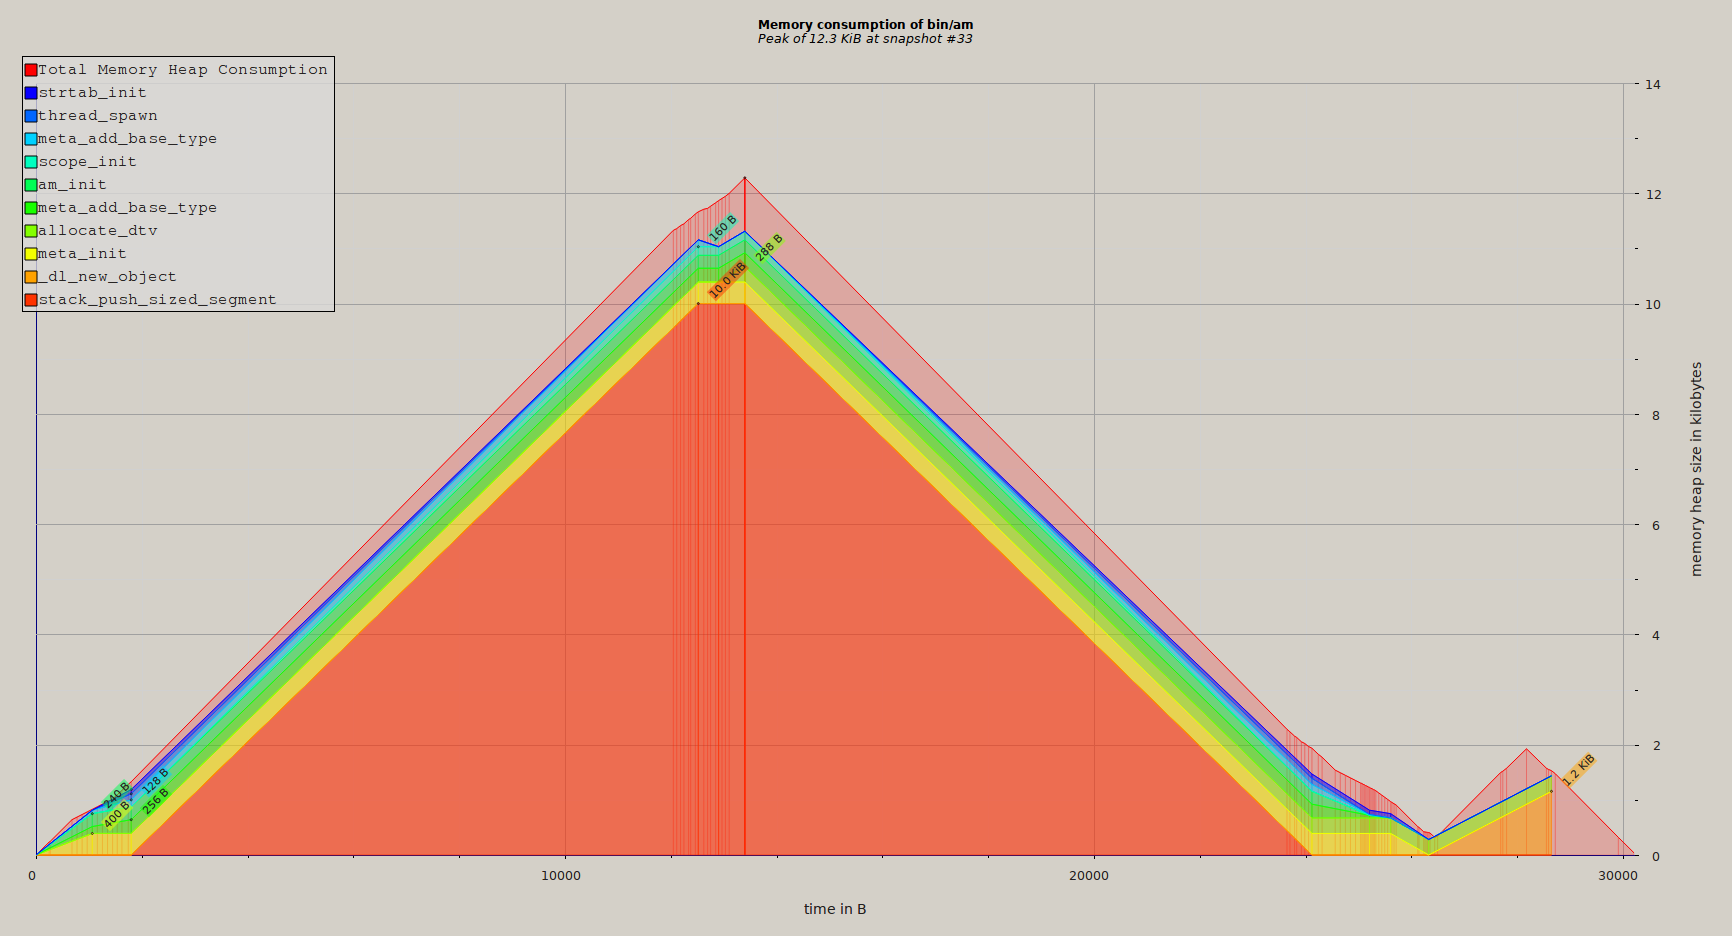
\includegraphics[scale=0.35]{figures/fig-mem}
  \caption{Heap profile of \thename{} running Fibonacci benchmark program}
\label{fig:heap-profile}
\end{figure}

The graph shows the memory heap size (in kB) on the y-axis and bytes allocated
and freed on the x-axis. Having the x-axis in bytes gives an alternative
representation of time, more beneficial when the actual running time is
irrelevant. Looking at the graph we see a pyramid shaped memory usage over the
duration of the program. The inner red fill of the pyramid is that used by the
the machine's stack, while the outer linings are information tables, threads
etc. This shows us that during start-up, memory is consumed by the information
tables and other core infrastructure, but following memory is solely consumed by
the stack. This makes good sense, as the Fibonacci benchmark does not mutate the
machine's state, with exception of the main thread's stack. The stack keeps
growing til half way into the program, and thereafter it declines at the same
pace. This pattern occurs because of how the Fibonacci program generates a very
deep recursion tree, as mentioned in the previous section. For each recursion,
two sub-routine invocations occur, resulting in two new activation frames being
pushed to the stack. When the the recursion tree finally ends in a leaf, the
value of $fib(n)$ is found, and the value is returned all the way up the
recursion tree, popping activation elements as it goes, until eventually being
returned to the original caller.

The result are indicating no unnecessary or unexpected use of memory.

\subsubsection{Optimization}

During the majority of the development we did not concern ourselves with
algorithmic optimization, but rather focused on designing suitable data
structures and writing maintainable and concise code that we would be able to
cope with the inevitable changes during the course of the project. As Rob Pike
states it in his first Rule of Programming: ``You can't tell where a program is
going to spend its time. Bottlenecks occur in surprising places, so don't try to
second guess and put in a speed hack until you've proven that's where the
bottleneck is.''\cite{pike-rules}. When the machine had reached a maturity level
that assured us that no further major changes to the overarching design were
necessary we started to analyze the code at a much more detailed level.

Memory leaks are extremely difficult to avoid when writing any non-trivial C
code. One has to meticulously track allocated memory chunks and free them at
just the right time and place to prevent invalid reads and writes. The fact that
C largely does not care about what some collection of bytes represents and
allows virtually any casting does not make this easier. One-off errors are
common when dealing with arrays and pointers which are indeed a central part of
the \thename{} implementation. Luckily there are tools available to aid in
profiling and pinpointing problematic parts of the code. Valgrind has been an
invaluable help for detecting memory errors and have allowed us to fix, to our
knowledge, all problematic leaks.

Valgrind consists of several different tools that analyze different things like
threads, stack operations, caches and memory. We have used the memory error
detector called Memcheck for finding leaks. When an executable is run through
Valgrind it is able to track allocations and the corresponding releases made
during the entire execution. If an allocation does not have exactly one
corresponding free operation it is either a leak or a double free (i.e.~a single
memory region attempted to be released more than once).

The output from Memcheck includes a list of errors and a summary of the leaked
amount of memory. When we initially ran Valgrind with the fibonacci test program
(with $n=15$) the leak summary was this:

\begin{verbatim}
==32067== LEAK SUMMARY:
==32067==    definitely lost: 410,033 bytes in 13,187 blocks
==32067==    indirectly lost: 371,808 bytes in 365 blocks
...
==32067== ERROR SUMMARY: 10 errors from 10 contexts (suppressed: 0 from 0)
\end{verbatim}

This says that there are 10 distinct errors causing a total leak of 400kB
memory, which is a very significant amount of memory for such a small and simple
program. Optimally there should be no bytes leaked at all. Valgrind also tells
you exactly where errors are introduced:

\begin{verbatim}
...
==32067== 27,608 bytes in 986 blocks are definitely lost in loss record 4 of 15
==32067==    at 0x4C29F90: malloc (in /usr/lib/valgrind/vgpreload_memcheck-amd64-linux.so)
==32067==    by 0x4018F4: stack_create_element (stack.c:128)
...
\end{verbatim}

An allocation is being made in the function \code{stack\_create\_element} and is
not released when the program exits. In this case we were not properly releasing
temporary stack elements, and being aware of the issue we changed the way stack
elements are created resulting in a sum total of 40 bytes leaked, all of which
are test data structures that are irrelevant for the actual performance
analysis. It is important to run multiple types of test programs through
Valgrind, because each of them may expose errors in differents parts of the
code.

The other form of profiling we did was by use of the equally great tool called
gprof\footnote{GNU gprof: \url{https://sourceware.org/binutils/docs/gprof/}}
(for GNU profiler). It works in a somewhat different way than Valgrind:
executables are compiled with a special profiling flag that injects profiling
code into the binary. When the file is executed it generates data that is then
run through gprof that performs the analysis. The output is a detailed overview
of the CPU time spent in each function. It is important to avoid profiling
optimized binaries because some crucial information can be lost when the
compiler performs various code transformations. For example, if the compiler
inlines a function into another, the former will appear to be using the
resources that are actually spent by the inlined function.

As an example of how we used gprof to pinpoint bottlenecks, an initial analysis
showed that 9\% of the total running time was spent in the function
\code{bytes2int} which converts a sequence of bytes into an integral C value. It
is a frequent operation but we found it is suspicious to be using almost one
tenth of the total CPU resources. It was indeed not optimally implemented;
Listing~\ref{lst:eval:gprof-pre} and~\ref{lst:eval:gprof-post} shows the
specific code before and after optimization.

\begin{minipage}{\linewidth}
\begin{lstlisting}[language={[ANSI]C},%
  caption={The function \code{bytes2int} before optimization.},%
  label={lst:eval:gprof-pre}]
int64_t value = 0;
int i = size;
while (i) {
    value += ((int64_t) bytes[i - 1]) << (8 * (size - i));
    i--;
}
return value;
\end{lstlisting}

\begin{lstlisting}[language={[ANSI]C},%
  caption={The function \code{bytes2int} after optimization},%
  label={lst:eval:gprof-post}]
switch (size) {
case 1: return bytes[0];
case 2: return bytes[1] | bytes[0] << 8;
case 4: return __builtin_bswap32(*(int32_t*)bytes);
case 8: return __builtin_bswap64(*(int64_t*)bytes);
default: return 0;
}
\end{lstlisting}
\end{minipage}

The optimized version of the function clocked in at the much better 1.4\% CPU
time. Using this technique of measuring, pinpointing, patching and measuring
again we managed to more than triple the speed of some test programs! Currently
the bottleneck of the machine seems to lie somewhere in the stack
implementation, as shown in the following gprof output:

\begin{verbatim}
  %   cumulative   self              self     total
 time   seconds   seconds    calls  ms/call  ms/call  name
 20.24      0.52     0.52 35002981     0.00     0.00  am_exec_instr
  8.17      0.73     0.21 24232831     0.00     0.00  stack_segment_push_element
  6.62      0.90     0.17 35002981     0.00     0.00  am_read_prefixes
  5.64      1.05     0.15 24232831     0.00     0.00  stack_push
  5.06      1.18     0.13 17501491     0.00     0.00  stack_peek
...
\end{verbatim}

Generally it is difficult to determine whether there is a problem with a part of
the code or if it is just a frequent operation in the specific
program. Profiling multiple test programs that utilize different features can
reveal common bottlenecks which should be analyzed further.

Whether there are more fundamental architectural design issues that limits
performance is difficult to say. We have not encountered major issues with how
the modules interoperate.

% JIT

A common form of optimization in modern abstract machines is the process of
compiling a program run-time, rather than prior to execution. As briefly
mentioned in Section~\ref{sec:background}, this technique is called just-in-time
compilation, or JIT.~This allows sections of code to be translated to machine
code which the host machine can execute directly. This is done just before the
code is going to be executed, hence the name. The translated machine code can
then be cached and reused. Therefore, if a function is called multiple times,
the machine can save time by paying the overhead of translating it to machine
code, but then saving time every time the same code is to be executed. A
challenge with JITing is balancing the overhead of translating to machine code
versus the saved time during execution. This overhead of just-in-time
compilation is called the ``startup time delay''.

In our earlier performance analysis, we have disabled all forms for such
optimizations to make the execution process of the different machines closer to
that of \thename{}. Figure~\ref{fig:eval:benchmark:jit} shows a benchmark of the
heap workout being run on JVM with and without JIT compilation.

\begin{figure}[H]
  \centering
  \scalebox{0.8}[0.6]{% Created by tikzDevice version 0.8.1 on 2015-06-28 21:11:30
% !TEX encoding = UTF-8 Unicode
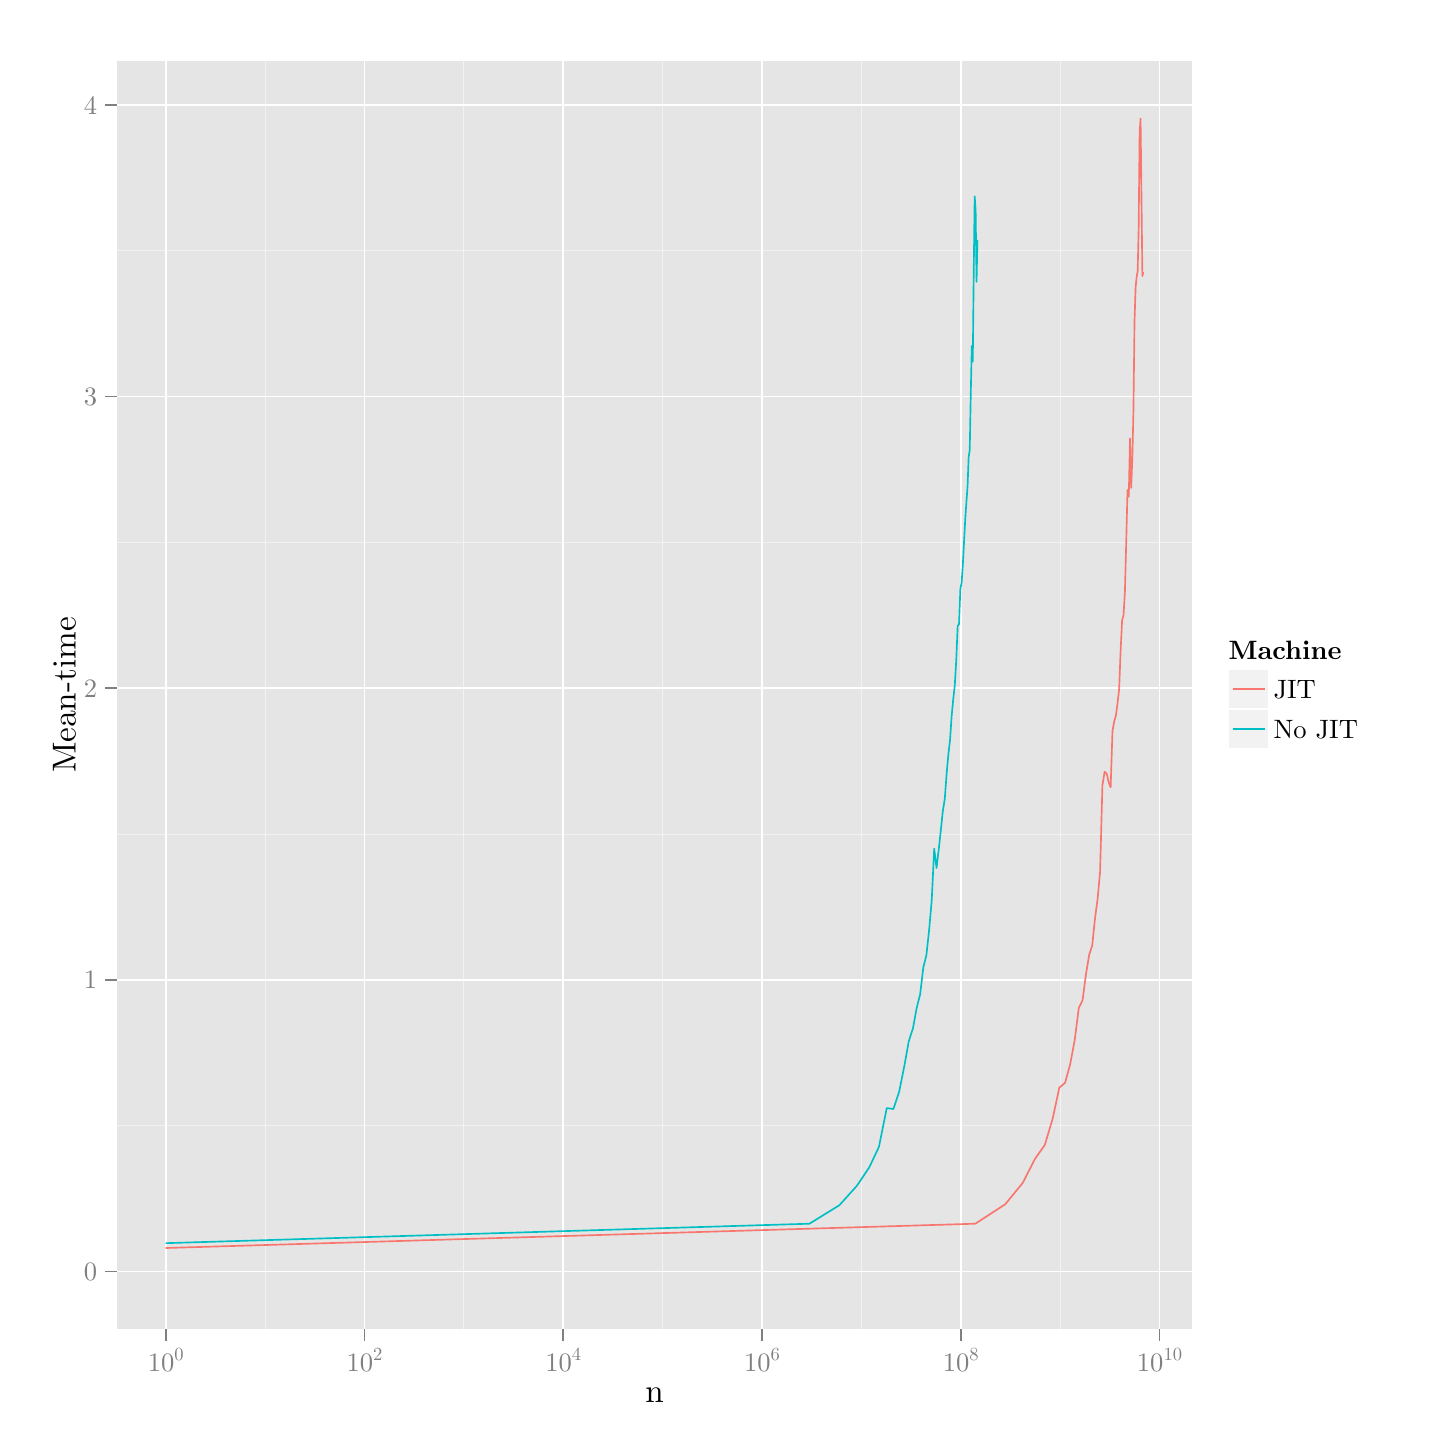
\begin{tikzpicture}[x=1pt,y=1pt]
\definecolor{fillColor}{RGB}{255,255,255}
\path[use as bounding box,fill=fillColor,fill opacity=0.00] (0,0) rectangle (505.89,505.89);
\begin{scope}
\path[clip] (  0.00,  0.00) rectangle (505.89,505.89);
\definecolor{drawColor}{RGB}{255,255,255}
\definecolor{fillColor}{RGB}{255,255,255}

\path[draw=drawColor,line width= 0.6pt,line join=round,line cap=round,fill=fillColor] (  0.00,  0.00) rectangle (505.89,505.89);
\end{scope}
\begin{scope}
\path[clip] ( 32.22, 35.66) rectangle (420.79,493.85);
\definecolor{fillColor}{gray}{0.90}

\path[fill=fillColor] ( 32.22, 35.66) rectangle (420.79,493.85);
\definecolor{drawColor}{gray}{0.95}

\path[draw=drawColor,line width= 0.3pt,line join=round] ( 32.22,109.17) --
	(420.79,109.17);

\path[draw=drawColor,line width= 0.3pt,line join=round] ( 32.22,214.53) --
	(420.79,214.53);

\path[draw=drawColor,line width= 0.3pt,line join=round] ( 32.22,319.89) --
	(420.79,319.89);

\path[draw=drawColor,line width= 0.3pt,line join=round] ( 32.22,425.25) --
	(420.79,425.25);

\path[draw=drawColor,line width= 0.3pt,line join=round] ( 85.80, 35.66) --
	( 85.80,493.85);

\path[draw=drawColor,line width= 0.3pt,line join=round] (157.62, 35.66) --
	(157.62,493.85);

\path[draw=drawColor,line width= 0.3pt,line join=round] (229.44, 35.66) --
	(229.44,493.85);

\path[draw=drawColor,line width= 0.3pt,line join=round] (301.27, 35.66) --
	(301.27,493.85);

\path[draw=drawColor,line width= 0.3pt,line join=round] (373.09, 35.66) --
	(373.09,493.85);
\definecolor{drawColor}{RGB}{255,255,255}

\path[draw=drawColor,line width= 0.6pt,line join=round] ( 32.22, 56.49) --
	(420.79, 56.49);

\path[draw=drawColor,line width= 0.6pt,line join=round] ( 32.22,161.85) --
	(420.79,161.85);

\path[draw=drawColor,line width= 0.6pt,line join=round] ( 32.22,267.21) --
	(420.79,267.21);

\path[draw=drawColor,line width= 0.6pt,line join=round] ( 32.22,372.57) --
	(420.79,372.57);

\path[draw=drawColor,line width= 0.6pt,line join=round] ( 32.22,477.94) --
	(420.79,477.94);

\path[draw=drawColor,line width= 0.6pt,line join=round] ( 49.88, 35.66) --
	( 49.88,493.85);

\path[draw=drawColor,line width= 0.6pt,line join=round] (121.71, 35.66) --
	(121.71,493.85);

\path[draw=drawColor,line width= 0.6pt,line join=round] (193.53, 35.66) --
	(193.53,493.85);

\path[draw=drawColor,line width= 0.6pt,line join=round] (265.36, 35.66) --
	(265.36,493.85);

\path[draw=drawColor,line width= 0.6pt,line join=round] (337.18, 35.66) --
	(337.18,493.85);

\path[draw=drawColor,line width= 0.6pt,line join=round] (409.00, 35.66) --
	(409.00,493.85);
\definecolor{drawColor}{RGB}{248,118,109}

\path[draw=drawColor,line width= 0.6pt,line join=round] ( 49.88, 64.92) --
	(342.43, 73.70) --
	(353.24, 80.72) --
	(359.56, 88.45) --
	(364.05, 97.23) --
	(367.53,102.14) --
	(370.37,111.63) --
	(372.78,122.86) --
	(374.86,124.62) --
	(376.70,131.29) --
	(378.34,140.07) --
	(379.82,151.66) --
	(381.18,154.47) --
	(382.43,163.96) --
	(383.59,170.98) --
	(384.66,174.14) --
	(385.67,183.97) --
	(386.61,191.00) --
	(387.51,200.83) --
	(388.35,232.09) --
	(389.15,237.01) --
	(389.91,236.30) --
	(390.64,233.14) --
	(391.33,231.39) --
	(391.99,251.76) --
	(392.63,255.27) --
	(393.24,257.38) --
	(393.83,261.94) --
	(394.40,266.86) --
	(394.94,280.91) --
	(395.47,291.80) --
	(395.98,293.55) --
	(396.48,301.98) --
	(396.96,320.24) --
	(397.42,338.86) --
	(397.88,336.40) --
	(398.32,357.47) --
	(398.74,339.56) --
	(399.16,350.10) --
	(399.56,367.30) --
	(399.96,399.97) --
	(400.34,411.91) --
	(400.72,415.77) --
	(401.09,417.88) --
	(401.45,433.33) --
	(401.80,468.10) --
	(402.14,473.02) --
	(402.47,444.57) --
	(402.80,416.12) --
	(403.12,417.53);
\definecolor{drawColor}{RGB}{0,191,196}

\path[draw=drawColor,line width= 0.6pt,line join=round] ( 49.88, 66.67) --
	(282.49, 73.70) --
	(293.30, 80.37) --
	(299.62, 87.39) --
	(304.11, 94.07) --
	(307.59,101.44) --
	(310.43,115.49) --
	(312.84,115.14) --
	(314.92,121.46) --
	(316.76,130.59) --
	(318.40,139.72) --
	(319.89,144.29) --
	(321.24,151.66) --
	(322.49,156.58) --
	(323.65,166.41) --
	(324.73,170.63) --
	(325.73,179.76) --
	(326.68,190.65) --
	(327.57,209.26) --
	(328.41,202.24) --
	(329.21,208.91) --
	(329.97,215.93) --
	(330.70,222.96) --
	(331.39,227.17) --
	(332.06,236.30) --
	(332.69,243.33) --
	(333.30,248.60) --
	(333.89,257.38) --
	(334.46,263.35) --
	(335.01,268.26) --
	(335.54,277.40) --
	(336.05,289.69) --
	(336.54,290.39) --
	(337.02,303.03) --
	(337.49,305.49) --
	(337.94,312.17) --
	(338.38,320.59) --
	(338.81,328.67) --
	(339.22,334.64) --
	(339.63,340.26) --
	(340.02,350.80) --
	(340.41,353.26) --
	(340.78,373.28) --
	(341.15,390.84) --
	(341.51,385.22) --
	(341.86,418.23) --
	(342.20,444.92) --
	(342.54,440.00) --
	(342.87,414.02) --
	(343.19,429.12);
\end{scope}
\begin{scope}
\path[clip] (  0.00,  0.00) rectangle (505.89,505.89);
\definecolor{drawColor}{gray}{0.50}

\node[text=drawColor,anchor=base east,inner sep=0pt, outer sep=0pt, scale=  0.96] at ( 25.11, 53.18) {0};

\node[text=drawColor,anchor=base east,inner sep=0pt, outer sep=0pt, scale=  0.96] at ( 25.11,158.54) {1};

\node[text=drawColor,anchor=base east,inner sep=0pt, outer sep=0pt, scale=  0.96] at ( 25.11,263.90) {2};

\node[text=drawColor,anchor=base east,inner sep=0pt, outer sep=0pt, scale=  0.96] at ( 25.11,369.27) {3};

\node[text=drawColor,anchor=base east,inner sep=0pt, outer sep=0pt, scale=  0.96] at ( 25.11,474.63) {4};
\end{scope}
\begin{scope}
\path[clip] (  0.00,  0.00) rectangle (505.89,505.89);
\definecolor{drawColor}{gray}{0.50}

\path[draw=drawColor,line width= 0.6pt,line join=round] ( 27.95, 56.49) --
	( 32.22, 56.49);

\path[draw=drawColor,line width= 0.6pt,line join=round] ( 27.95,161.85) --
	( 32.22,161.85);

\path[draw=drawColor,line width= 0.6pt,line join=round] ( 27.95,267.21) --
	( 32.22,267.21);

\path[draw=drawColor,line width= 0.6pt,line join=round] ( 27.95,372.57) --
	( 32.22,372.57);

\path[draw=drawColor,line width= 0.6pt,line join=round] ( 27.95,477.94) --
	( 32.22,477.94);
\end{scope}
\begin{scope}
\path[clip] (  0.00,  0.00) rectangle (505.89,505.89);
\definecolor{drawColor}{gray}{0.50}

\path[draw=drawColor,line width= 0.6pt,line join=round] ( 49.88, 31.39) --
	( 49.88, 35.66);

\path[draw=drawColor,line width= 0.6pt,line join=round] (121.71, 31.39) --
	(121.71, 35.66);

\path[draw=drawColor,line width= 0.6pt,line join=round] (193.53, 31.39) --
	(193.53, 35.66);

\path[draw=drawColor,line width= 0.6pt,line join=round] (265.36, 31.39) --
	(265.36, 35.66);

\path[draw=drawColor,line width= 0.6pt,line join=round] (337.18, 31.39) --
	(337.18, 35.66);

\path[draw=drawColor,line width= 0.6pt,line join=round] (409.00, 31.39) --
	(409.00, 35.66);
\end{scope}
\begin{scope}
\path[clip] (  0.00,  0.00) rectangle (505.89,505.89);
\definecolor{drawColor}{gray}{0.50}

\node[text=drawColor,anchor=base west,inner sep=0pt, outer sep=0pt, scale=  0.96] at ( 43.41, 20.31) {10};

\node[text=drawColor,anchor=base west,inner sep=0pt, outer sep=0pt, scale=  0.67] at ( 53.00, 24.24) {0};

\node[text=drawColor,anchor=base west,inner sep=0pt, outer sep=0pt, scale=  0.96] at (115.23, 20.31) {10};

\node[text=drawColor,anchor=base west,inner sep=0pt, outer sep=0pt, scale=  0.67] at (124.83, 24.24) {2};

\node[text=drawColor,anchor=base west,inner sep=0pt, outer sep=0pt, scale=  0.96] at (187.05, 20.31) {10};

\node[text=drawColor,anchor=base west,inner sep=0pt, outer sep=0pt, scale=  0.67] at (196.65, 24.24) {4};

\node[text=drawColor,anchor=base west,inner sep=0pt, outer sep=0pt, scale=  0.96] at (258.88, 20.31) {10};

\node[text=drawColor,anchor=base west,inner sep=0pt, outer sep=0pt, scale=  0.67] at (268.47, 24.24) {6};

\node[text=drawColor,anchor=base west,inner sep=0pt, outer sep=0pt, scale=  0.96] at (330.70, 20.31) {10};

\node[text=drawColor,anchor=base west,inner sep=0pt, outer sep=0pt, scale=  0.67] at (340.30, 24.24) {8};

\node[text=drawColor,anchor=base west,inner sep=0pt, outer sep=0pt, scale=  0.96] at (400.84, 20.31) {10};

\node[text=drawColor,anchor=base west,inner sep=0pt, outer sep=0pt, scale=  0.67] at (410.44, 24.24) {1};

\node[text=drawColor,anchor=base west,inner sep=0pt, outer sep=0pt, scale=  0.67] at (413.80, 24.24) {0};
\end{scope}
\begin{scope}
\path[clip] (  0.00,  0.00) rectangle (505.89,505.89);
\definecolor{drawColor}{RGB}{0,0,0}

\node[text=drawColor,anchor=base,inner sep=0pt, outer sep=0pt, scale=  1.20] at (226.50,  9.03) {n};
\end{scope}
\begin{scope}
\path[clip] (  0.00,  0.00) rectangle (505.89,505.89);
\definecolor{drawColor}{RGB}{0,0,0}

\node[text=drawColor,rotate= 90.00,anchor=base,inner sep=0pt, outer sep=0pt, scale=  1.20] at ( 17.30,264.75) {Mean-time};
\end{scope}
\begin{scope}
\path[clip] (  0.00,  0.00) rectangle (505.89,505.89);
\definecolor{fillColor}{RGB}{255,255,255}

\path[fill=fillColor] (429.65,240.91) rectangle (484.98,288.59);
\end{scope}
\begin{scope}
\path[clip] (  0.00,  0.00) rectangle (505.89,505.89);
\definecolor{drawColor}{RGB}{0,0,0}

\node[text=drawColor,anchor=base west,inner sep=0pt, outer sep=0pt, scale=  0.96] at (433.92,277.70) {\bfseries Machine};
\end{scope}
\begin{scope}
\path[clip] (  0.00,  0.00) rectangle (505.89,505.89);
\definecolor{drawColor}{RGB}{255,255,255}
\definecolor{fillColor}{gray}{0.95}

\path[draw=drawColor,line width= 0.6pt,line join=round,line cap=round,fill=fillColor] (433.92,259.63) rectangle (448.38,274.09);
\end{scope}
\begin{scope}
\path[clip] (  0.00,  0.00) rectangle (505.89,505.89);
\definecolor{drawColor}{RGB}{248,118,109}

\path[draw=drawColor,line width= 0.6pt,line join=round] (435.37,266.86) -- (446.93,266.86);
\end{scope}
\begin{scope}
\path[clip] (  0.00,  0.00) rectangle (505.89,505.89);
\definecolor{drawColor}{RGB}{255,255,255}
\definecolor{fillColor}{gray}{0.95}

\path[draw=drawColor,line width= 0.6pt,line join=round,line cap=round,fill=fillColor] (433.92,245.18) rectangle (448.38,259.63);
\end{scope}
\begin{scope}
\path[clip] (  0.00,  0.00) rectangle (505.89,505.89);
\definecolor{drawColor}{RGB}{0,191,196}

\path[draw=drawColor,line width= 0.6pt,line join=round] (435.37,252.41) -- (446.93,252.41);
\end{scope}
\begin{scope}
\path[clip] (  0.00,  0.00) rectangle (505.89,505.89);
\definecolor{drawColor}{RGB}{0,0,0}

\node[text=drawColor,anchor=base west,inner sep=0pt, outer sep=0pt, scale=  0.96] at (450.18,263.55) {JIT};
\end{scope}
\begin{scope}
\path[clip] (  0.00,  0.00) rectangle (505.89,505.89);
\definecolor{drawColor}{RGB}{0,0,0}

\node[text=drawColor,anchor=base west,inner sep=0pt, outer sep=0pt, scale=  0.96] at (450.18,249.10) {No JIT};
\end{scope}
\end{tikzpicture}
}
  \caption{JIT comparing on JVM}
\label{fig:eval:benchmark:jit}
\end{figure}

The benefit of JIT compilation is striking, it runs more than an order of
magnitude faster. Even with small numbers, we see that the statup time delay
that occurs when using JIT is still outweighed by the faster execution
time. This is obviously a very simple program which means that the JIT process
will be very short, and thus the cost of JITting is most certainly higher for
larger programs.

\subsection{Code Analysis}

Another side of code evaluation is to view the source code from a macro
perspective, including trivial things such as counting source lines of code
(SLOC) and looking at the number of comments per line of
code. Figure~\ref{fig:eval:sloc} shows the division of code in the source
directory and in the tests. The amount of source code is well correlated with
the amount of work performed by each module. The test SLOC are not proportional
to the amount of code in the corresponding module because some algorithms
require much more extensive unit tests than others. For instance the type
conversion algorithms must cover almost all different combinations of types
which results in extensive tests.

\begin{figure}
  \centering
  % Created by tikzDevice version 0.8.1 on 2015-06-28 21:35:40
% !TEX encoding = UTF-8 Unicode
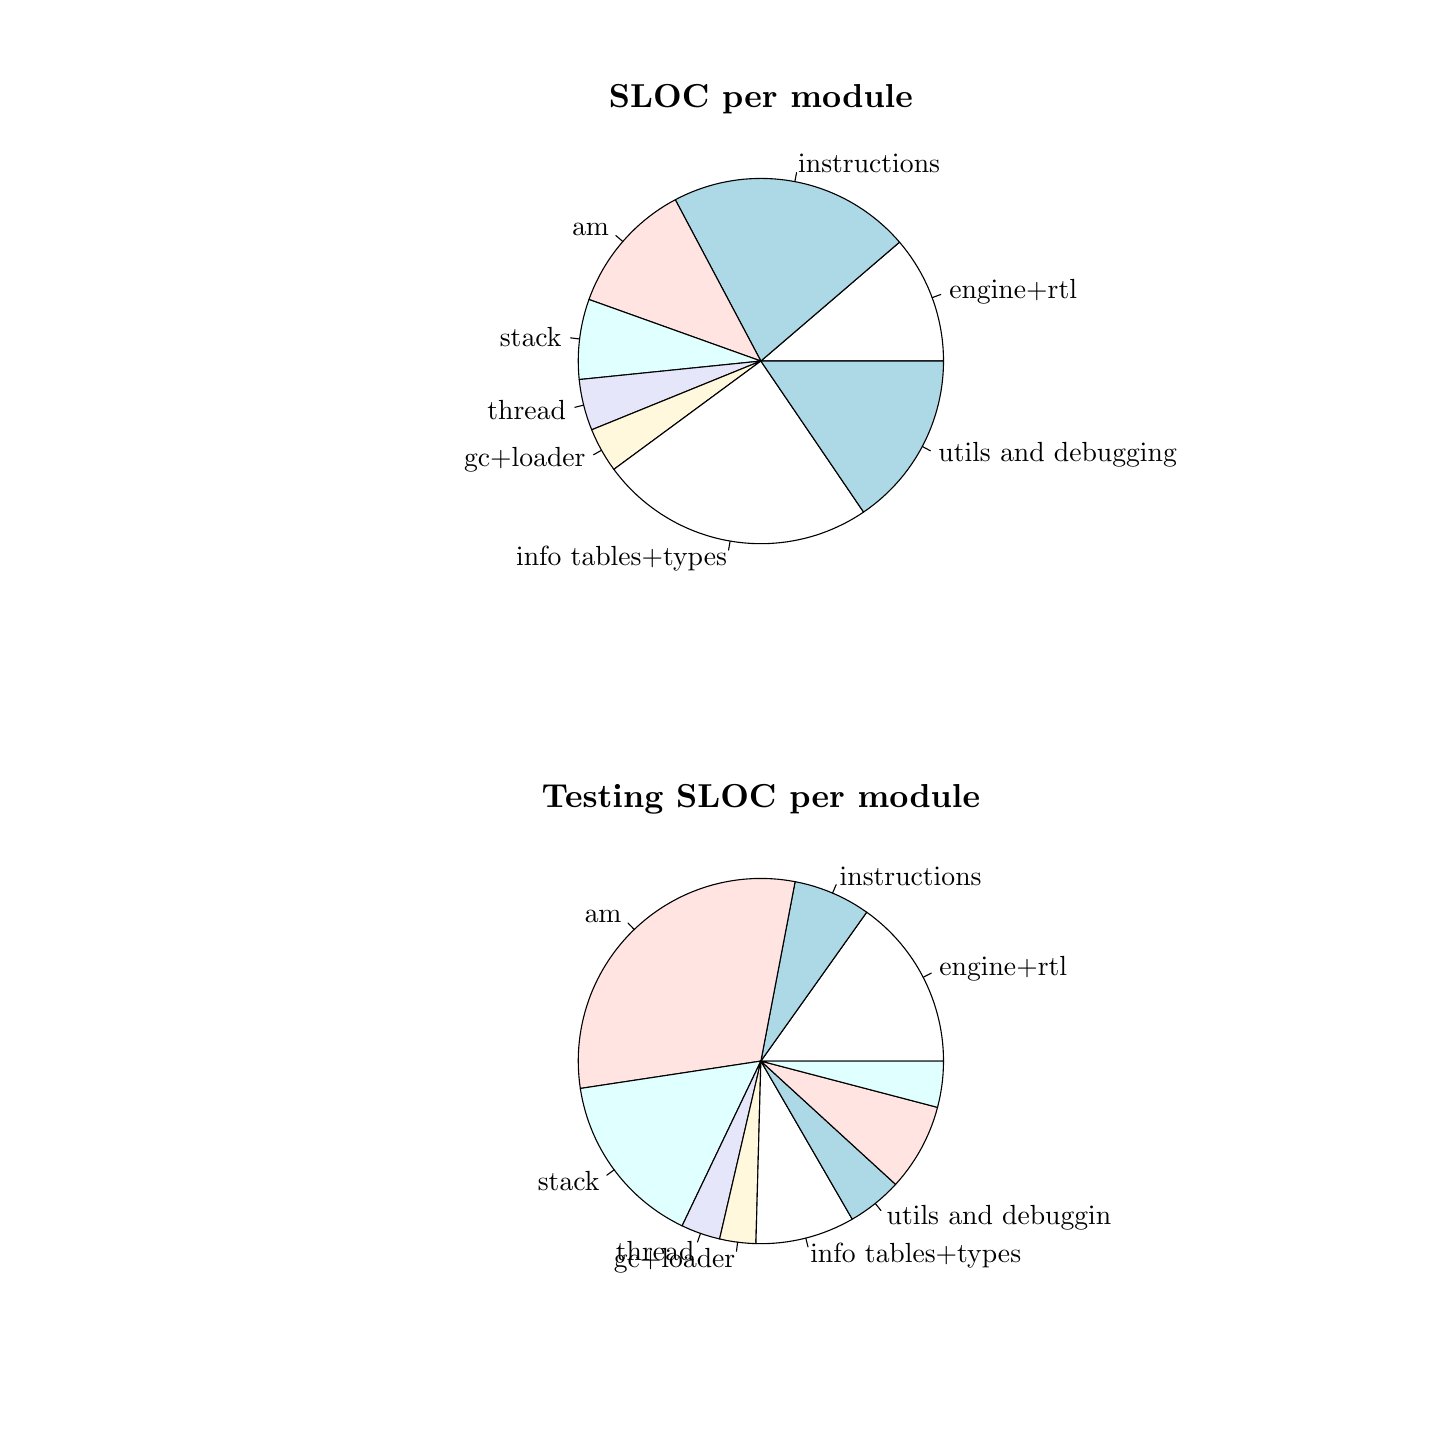
\begin{tikzpicture}[x=1pt,y=1pt]
\definecolor{fillColor}{RGB}{255,255,255}
\path[use as bounding box,fill=fillColor,fill opacity=0.00] (0,0) rectangle (505.89,505.89);
\begin{scope}
\path[clip] ( 49.20,314.14) rectangle (480.69,456.69);
\definecolor{drawColor}{RGB}{0,0,0}
\definecolor{fillColor}{RGB}{255,255,255}

\path[draw=drawColor,line width= 0.4pt,line join=round,line cap=round,fill=fillColor] (330.94,385.42) --
	(330.90,387.64) --
	(330.79,389.87) --
	(330.60,392.09) --
	(330.34,394.30) --
	(330.00,396.50) --
	(329.59,398.69) --
	(329.10,400.87) --
	(328.55,403.02) --
	(327.92,405.16) --
	(327.21,407.27) --
	(326.44,409.36) --
	(325.60,411.43) --
	(324.68,413.46) --
	(323.70,415.46) --
	(322.66,417.42) --
	(321.54,419.35) --
	(320.37,421.24) --
	(319.13,423.09) --
	(317.82,424.90) --
	(316.46,426.66) --
	(315.04,428.38) --
	(264.94,385.42) --
	cycle;

\path[draw=drawColor,line width= 0.4pt,line join=round,line cap=round] (326.84,408.32) --
	(329.93,409.47);
\end{scope}
\begin{scope}
\path[clip] (  0.00,252.94) rectangle (505.89,505.89);
\definecolor{drawColor}{RGB}{0,0,0}

\node[text=drawColor,anchor=base west,inner sep=0pt, outer sep=0pt, scale=  1.00] at (333.02,408.14) {engine+rtl};
\end{scope}
\begin{scope}
\path[clip] ( 49.20,314.14) rectangle (480.69,456.69);
\definecolor{drawColor}{RGB}{0,0,0}
\definecolor{fillColor}{RGB}{173,216,230}

\path[draw=drawColor,line width= 0.4pt,line join=round,line cap=round,fill=fillColor] (315.04,428.38) --
	(313.60,430.00) --
	(312.10,431.58) --
	(310.56,433.11) --
	(308.96,434.58) --
	(307.32,436.01) --
	(305.63,437.37) --
	(303.90,438.68) --
	(302.13,439.94) --
	(300.31,441.13) --
	(298.46,442.27) --
	(296.57,443.34) --
	(294.65,444.35) --
	(292.69,445.29) --
	(290.71,446.17) --
	(288.69,446.99) --
	(286.65,447.74) --
	(284.59,448.42) --
	(282.51,449.03) --
	(280.40,449.57) --
	(278.28,450.05) --
	(276.15,450.45) --
	(274.00,450.79) --
	(271.85,451.05) --
	(269.68,451.24) --
	(267.51,451.36) --
	(265.34,451.41) --
	(263.17,451.39) --
	(261.00,451.29) --
	(258.83,451.13) --
	(256.67,450.89) --
	(254.52,450.58) --
	(252.38,450.20) --
	(250.26,449.76) --
	(248.15,449.24) --
	(246.06,448.65) --
	(243.99,447.99) --
	(241.94,447.27) --
	(239.91,446.48) --
	(237.92,445.62) --
	(235.95,444.70) --
	(234.02,443.71) --
	(264.94,385.42) --
	cycle;

\path[draw=drawColor,line width= 0.4pt,line join=round,line cap=round] (277.22,450.26) --
	(277.83,453.50);
\end{scope}
\begin{scope}
\path[clip] (  0.00,252.94) rectangle (505.89,505.89);
\definecolor{drawColor}{RGB}{0,0,0}

\node[text=drawColor,anchor=base west,inner sep=0pt, outer sep=0pt, scale=  1.00] at (278.44,453.43) {instructions};
\end{scope}
\begin{scope}
\path[clip] ( 49.20,314.14) rectangle (480.69,456.69);
\definecolor{drawColor}{RGB}{0,0,0}
\definecolor{fillColor}{RGB}{255,228,225}

\path[draw=drawColor,line width= 0.4pt,line join=round,line cap=round,fill=fillColor] (234.02,443.71) --
	(232.08,442.64) --
	(230.17,441.51) --
	(228.31,440.31) --
	(226.49,439.05) --
	(224.71,437.72) --
	(222.97,436.34) --
	(221.28,434.90) --
	(219.65,433.41) --
	(218.06,431.86) --
	(216.53,430.26) --
	(215.05,428.61) --
	(213.63,426.91) --
	(212.26,425.16) --
	(210.96,423.37) --
	(209.71,421.53) --
	(208.53,419.66) --
	(207.41,417.75) --
	(206.36,415.79) --
	(205.37,413.81) --
	(204.45,411.79) --
	(203.60,409.75) --
	(202.82,407.67) --
	(264.94,385.42) --
	cycle;

\path[draw=drawColor,line width= 0.4pt,line join=round,line cap=round] (215.05,428.61) --
	(212.55,430.77);
\end{scope}
\begin{scope}
\path[clip] (  0.00,252.94) rectangle (505.89,505.89);
\definecolor{drawColor}{RGB}{0,0,0}

\node[text=drawColor,anchor=base east,inner sep=0pt, outer sep=0pt, scale=  1.00] at (210.06,430.78) {am};
\end{scope}
\begin{scope}
\path[clip] ( 49.20,314.14) rectangle (480.69,456.69);
\definecolor{drawColor}{RGB}{0,0,0}
\definecolor{fillColor}{RGB}{224,255,255}

\path[draw=drawColor,line width= 0.4pt,line join=round,line cap=round,fill=fillColor] (202.82,407.67) --
	(202.09,405.53) --
	(201.44,403.36) --
	(200.86,401.18) --
	(200.36,398.97) --
	(199.93,396.75) --
	(199.58,394.52) --
	(199.31,392.27) --
	(199.11,390.02) --
	(198.99,387.76) --
	(198.95,385.50) --
	(198.99,383.24) --
	(199.10,380.98) --
	(199.29,378.73) --
	(264.94,385.42) --
	cycle;

\path[draw=drawColor,line width= 0.4pt,line join=round,line cap=round] (199.44,393.40) --
	(196.16,393.80);
\end{scope}
\begin{scope}
\path[clip] (  0.00,252.94) rectangle (505.89,505.89);
\definecolor{drawColor}{RGB}{0,0,0}

\node[text=drawColor,anchor=base east,inner sep=0pt, outer sep=0pt, scale=  1.00] at (192.89,390.75) {stack};
\end{scope}
\begin{scope}
\path[clip] ( 49.20,314.14) rectangle (480.69,456.69);
\definecolor{drawColor}{RGB}{0,0,0}
\definecolor{fillColor}{RGB}{230,230,250}

\path[draw=drawColor,line width= 0.4pt,line join=round,line cap=round,fill=fillColor] (199.29,378.73) --
	(199.57,376.40) --
	(199.93,374.08) --
	(200.38,371.78) --
	(200.90,369.49) --
	(201.51,367.23) --
	(202.20,364.98) --
	(202.96,362.77) --
	(203.81,360.58) --
	(264.94,385.42) --
	cycle;

\path[draw=drawColor,line width= 0.4pt,line join=round,line cap=round] (200.90,369.49) --
	(197.70,368.70);
\end{scope}
\begin{scope}
\path[clip] (  0.00,252.94) rectangle (505.89,505.89);
\definecolor{drawColor}{RGB}{0,0,0}

\node[text=drawColor,anchor=base east,inner sep=0pt, outer sep=0pt, scale=  1.00] at (194.50,364.46) {thread};
\end{scope}
\begin{scope}
\path[clip] ( 49.20,314.14) rectangle (480.69,456.69);
\definecolor{drawColor}{RGB}{0,0,0}
\definecolor{fillColor}{RGB}{255,248,220}

\path[draw=drawColor,line width= 0.4pt,line join=round,line cap=round,fill=fillColor] (203.81,360.58) --
	(204.89,358.06) --
	(206.07,355.60) --
	(207.36,353.18) --
	(208.75,350.82) --
	(210.23,348.52) --
	(211.81,346.28) --
	(264.94,385.42) --
	cycle;

\path[draw=drawColor,line width= 0.4pt,line join=round,line cap=round] (207.36,353.18) --
	(204.48,351.57);
\end{scope}
\begin{scope}
\path[clip] (  0.00,252.94) rectangle (505.89,505.89);
\definecolor{drawColor}{RGB}{0,0,0}

\node[text=drawColor,anchor=base east,inner sep=0pt, outer sep=0pt, scale=  1.00] at (201.60,347.48) {gc+loader};
\end{scope}
\begin{scope}
\path[clip] ( 49.20,314.14) rectangle (480.69,456.69);
\definecolor{drawColor}{RGB}{0,0,0}
\definecolor{fillColor}{RGB}{255,255,255}

\path[draw=drawColor,line width= 0.4pt,line join=round,line cap=round,fill=fillColor] (211.81,346.28) --
	(213.12,344.57) --
	(214.48,342.90) --
	(215.89,341.27) --
	(217.35,339.70) --
	(218.87,338.17) --
	(220.44,336.69) --
	(222.05,335.27) --
	(223.71,333.89) --
	(225.41,332.58) --
	(227.15,331.32) --
	(228.94,330.11) --
	(230.76,328.97) --
	(232.62,327.88) --
	(234.51,326.86) --
	(236.44,325.90) --
	(238.40,325.00) --
	(240.38,324.17) --
	(242.39,323.40) --
	(244.43,322.70) --
	(246.48,322.06) --
	(248.56,321.49) --
	(250.65,320.99) --
	(252.76,320.56) --
	(254.88,320.20) --
	(257.02,319.90) --
	(259.16,319.68) --
	(261.30,319.52) --
	(263.46,319.44) --
	(265.61,319.43) --
	(267.76,319.48) --
	(269.91,319.61) --
	(272.05,319.81) --
	(274.19,320.07) --
	(276.31,320.41) --
	(278.43,320.82) --
	(280.53,321.29) --
	(282.61,321.83) --
	(284.68,322.44) --
	(286.72,323.12) --
	(288.74,323.86) --
	(290.73,324.67) --
	(292.70,325.55) --
	(294.64,326.48) --
	(296.55,327.48) --
	(298.42,328.54) --
	(300.26,329.67) --
	(302.05,330.85) --
	(264.94,385.42) --
	cycle;

\path[draw=drawColor,line width= 0.4pt,line join=round,line cap=round] (253.82,320.37) --
	(253.27,317.12);
\end{scope}
\begin{scope}
\path[clip] (  0.00,252.94) rectangle (505.89,505.89);
\definecolor{drawColor}{RGB}{0,0,0}

\node[text=drawColor,anchor=base east,inner sep=0pt, outer sep=0pt, scale=  1.00] at (252.71,311.39) {info tables+types};
\end{scope}
\begin{scope}
\path[clip] ( 49.20,314.14) rectangle (480.69,456.69);
\definecolor{drawColor}{RGB}{0,0,0}
\definecolor{fillColor}{RGB}{173,216,230}

\path[draw=drawColor,line width= 0.4pt,line join=round,line cap=round,fill=fillColor] (302.05,330.85) --
	(303.87,332.12) --
	(305.63,333.46) --
	(307.35,334.85) --
	(309.03,336.31) --
	(310.65,337.81) --
	(312.22,339.37) --
	(313.74,340.99) --
	(315.21,342.65) --
	(316.61,344.36) --
	(317.96,346.12) --
	(319.25,347.92) --
	(320.48,349.76) --
	(321.64,351.65) --
	(322.75,353.57) --
	(323.78,355.53) --
	(324.75,357.52) --
	(325.65,359.54) --
	(326.49,361.60) --
	(327.25,363.68) --
	(327.95,365.78) --
	(328.57,367.91) --
	(329.12,370.05) --
	(329.60,372.21) --
	(330.01,374.39) --
	(330.34,376.58) --
	(330.60,378.78) --
	(330.79,380.99) --
	(330.90,383.20) --
	(330.94,385.42) --
	(264.94,385.42) --
	cycle;

\path[draw=drawColor,line width= 0.4pt,line join=round,line cap=round] (323.27,354.55) --
	(326.19,353.00);
\end{scope}
\begin{scope}
\path[clip] (  0.00,252.94) rectangle (505.89,505.89);
\definecolor{drawColor}{RGB}{0,0,0}

\node[text=drawColor,anchor=base west,inner sep=0pt, outer sep=0pt, scale=  1.00] at (329.10,348.99) {utils and debugging};

\node[text=drawColor,anchor=base,inner sep=0pt, outer sep=0pt, scale=  1.20] at (264.94,477.15) {\bfseries SLOC per module};
\end{scope}
\begin{scope}
\path[clip] ( 49.20, 61.20) rectangle (480.69,203.75);
\definecolor{drawColor}{RGB}{0,0,0}
\definecolor{fillColor}{RGB}{255,255,255}

\path[draw=drawColor,line width= 0.4pt,line join=round,line cap=round,fill=fillColor] (330.94,132.47) --
	(330.90,134.64) --
	(330.80,136.81) --
	(330.62,138.97) --
	(330.37,141.12) --
	(330.05,143.27) --
	(329.66,145.40) --
	(329.20,147.52) --
	(328.67,149.62) --
	(328.07,151.70) --
	(327.41,153.77) --
	(326.67,155.81) --
	(325.87,157.82) --
	(325.01,159.81) --
	(324.08,161.77) --
	(323.08,163.70) --
	(322.03,165.59) --
	(320.91,167.45) --
	(319.73,169.27) --
	(318.49,171.05) --
	(317.19,172.78) --
	(315.84,174.48) --
	(314.44,176.13) --
	(312.97,177.73) --
	(311.46,179.28) --
	(309.90,180.79) --
	(308.29,182.24) --
	(306.63,183.63) --
	(304.93,184.98) --
	(303.18,186.26) --
	(264.94,132.47) --
	cycle;

\path[draw=drawColor,line width= 0.4pt,line join=round,line cap=round] (323.59,162.74) --
	(326.52,164.25);
\end{scope}
\begin{scope}
\path[clip] (  0.00,  0.00) rectangle (505.89,252.94);
\definecolor{drawColor}{RGB}{0,0,0}

\node[text=drawColor,anchor=base west,inner sep=0pt, outer sep=0pt, scale=  1.00] at (329.45,163.29) {engine+rtl};
\end{scope}
\begin{scope}
\path[clip] ( 49.20, 61.20) rectangle (480.69,203.75);
\definecolor{drawColor}{RGB}{0,0,0}
\definecolor{fillColor}{RGB}{173,216,230}

\path[draw=drawColor,line width= 0.4pt,line join=round,line cap=round,fill=fillColor] (303.18,186.26) --
	(301.23,187.59) --
	(299.24,188.86) --
	(297.20,190.05) --
	(295.12,191.17) --
	(293.00,192.21) --
	(290.84,193.17) --
	(288.65,194.06) --
	(286.43,194.87) --
	(284.19,195.60) --
	(281.92,196.25) --
	(279.62,196.81) --
	(277.31,197.30) --
	(264.94,132.47) --
	cycle;

\path[draw=drawColor,line width= 0.4pt,line join=round,line cap=round] (290.84,193.17) --
	(292.14,196.21);
\end{scope}
\begin{scope}
\path[clip] (  0.00,  0.00) rectangle (505.89,252.94);
\definecolor{drawColor}{RGB}{0,0,0}

\node[text=drawColor,anchor=base west,inner sep=0pt, outer sep=0pt, scale=  1.00] at (293.43,195.93) {instructions};
\end{scope}
\begin{scope}
\path[clip] ( 49.20, 61.20) rectangle (480.69,203.75);
\definecolor{drawColor}{RGB}{0,0,0}
\definecolor{fillColor}{RGB}{255,228,225}

\path[draw=drawColor,line width= 0.4pt,line join=round,line cap=round,fill=fillColor] (277.31,197.30) --
	(275.21,197.66) --
	(273.09,197.96) --
	(270.97,198.19) --
	(268.84,198.35) --
	(266.71,198.44) --
	(264.57,198.46) --
	(262.43,198.42) --
	(260.30,198.30) --
	(258.17,198.12) --
	(256.05,197.86) --
	(253.94,197.54) --
	(251.84,197.15) --
	(249.75,196.69) --
	(247.68,196.17) --
	(245.63,195.58) --
	(243.60,194.92) --
	(241.59,194.19) --
	(239.60,193.41) --
	(237.64,192.55) --
	(235.71,191.64) --
	(233.81,190.66) --
	(231.95,189.62) --
	(230.11,188.52) --
	(228.32,187.37) --
	(226.56,186.15) --
	(224.84,184.88) --
	(223.17,183.56) --
	(221.54,182.18) --
	(219.95,180.75) --
	(218.41,179.27) --
	(216.92,177.74) --
	(215.48,176.16) --
	(214.09,174.53) --
	(212.76,172.87) --
	(211.48,171.16) --
	(210.25,169.40) --
	(209.09,167.61) --
	(207.98,165.79) --
	(206.93,163.93) --
	(205.94,162.03) --
	(205.02,160.11) --
	(204.15,158.15) --
	(203.35,156.17) --
	(202.62,154.17) --
	(201.95,152.14) --
	(201.35,150.09) --
	(200.81,148.02) --
	(200.34,145.94) --
	(199.94,143.84) --
	(199.60,141.73) --
	(199.34,139.61) --
	(199.14,137.48) --
	(199.01,135.35) --
	(198.96,133.21) --
	(198.97,131.08) --
	(199.05,128.94) --
	(199.20,126.81) --
	(199.41,124.69) --
	(199.70,122.57) --
	(264.94,132.47) --
	cycle;

\path[draw=drawColor,line width= 0.4pt,line join=round,line cap=round] (219.17,180.01) --
	(216.89,182.39);
\end{scope}
\begin{scope}
\path[clip] (  0.00,  0.00) rectangle (505.89,252.94);
\definecolor{drawColor}{RGB}{0,0,0}

\node[text=drawColor,anchor=base east,inner sep=0pt, outer sep=0pt, scale=  1.00] at (214.60,182.61) {am};
\end{scope}
\begin{scope}
\path[clip] ( 49.20, 61.20) rectangle (480.69,203.75);
\definecolor{drawColor}{RGB}{0,0,0}
\definecolor{fillColor}{RGB}{224,255,255}

\path[draw=drawColor,line width= 0.4pt,line join=round,line cap=round,fill=fillColor] (199.70,122.57) --
	(200.05,120.46) --
	(200.48,118.36) --
	(200.97,116.27) --
	(201.53,114.20) --
	(202.16,112.15) --
	(202.85,110.13) --
	(203.61,108.12) --
	(204.43,106.14) --
	(205.32,104.19) --
	(206.27,102.27) --
	(207.28,100.38) --
	(208.35, 98.53) --
	(209.48, 96.71) --
	(210.67, 94.92) --
	(211.92, 93.18) --
	(213.23, 91.48) --
	(214.58, 89.82) --
	(216.00, 88.21) --
	(217.46, 86.65) --
	(218.97, 85.13) --
	(220.53, 83.66) --
	(222.14, 82.24) --
	(223.79, 80.88) --
	(225.49, 79.57) --
	(227.23, 78.32) --
	(229.01, 77.12) --
	(230.82, 75.99) --
	(232.68, 74.91) --
	(234.56, 73.89) --
	(236.48, 72.93) --
	(264.94,132.47) --
	cycle;

\path[draw=drawColor,line width= 0.4pt,line join=round,line cap=round] (211.92, 93.18) --
	(209.27, 91.22);
\end{scope}
\begin{scope}
\path[clip] (  0.00,  0.00) rectangle (505.89,252.94);
\definecolor{drawColor}{RGB}{0,0,0}

\node[text=drawColor,anchor=base east,inner sep=0pt, outer sep=0pt, scale=  1.00] at (206.62, 85.81) {stack};
\end{scope}
\begin{scope}
\path[clip] ( 49.20, 61.20) rectangle (480.69,203.75);
\definecolor{drawColor}{RGB}{0,0,0}
\definecolor{fillColor}{RGB}{230,230,250}

\path[draw=drawColor,line width= 0.4pt,line join=round,line cap=round,fill=fillColor] (236.48, 72.93) --
	(239.10, 71.75) --
	(241.77, 70.68) --
	(244.48, 69.73) --
	(247.24, 68.90) --
	(250.02, 68.19) --
	(264.94,132.47) --
	cycle;

\path[draw=drawColor,line width= 0.4pt,line join=round,line cap=round] (243.12, 70.19) --
	(242.03, 67.08);
\end{scope}
\begin{scope}
\path[clip] (  0.00,  0.00) rectangle (505.89,252.94);
\definecolor{drawColor}{RGB}{0,0,0}

\node[text=drawColor,anchor=base east,inner sep=0pt, outer sep=0pt, scale=  1.00] at (240.94, 60.52) {thread};
\end{scope}
\begin{scope}
\path[clip] ( 49.20, 61.20) rectangle (480.69,203.75);
\definecolor{drawColor}{RGB}{0,0,0}
\definecolor{fillColor}{RGB}{255,248,220}

\path[draw=drawColor,line width= 0.4pt,line join=round,line cap=round,fill=fillColor] (250.02, 68.19) --
	(252.62, 67.64) --
	(255.23, 67.20) --
	(257.86, 66.86) --
	(260.50, 66.63) --
	(263.15, 66.50) --
	(264.94,132.47) --
	cycle;

\path[draw=drawColor,line width= 0.4pt,line join=round,line cap=round] (256.54, 67.02) --
	(256.12, 63.74);
\end{scope}
\begin{scope}
\path[clip] (  0.00,  0.00) rectangle (505.89,252.94);
\definecolor{drawColor}{RGB}{0,0,0}

\node[text=drawColor,anchor=base east,inner sep=0pt, outer sep=0pt, scale=  1.00] at (255.70, 58.00) {gc+loader};
\end{scope}
\begin{scope}
\path[clip] ( 49.20, 61.20) rectangle (480.69,203.75);
\definecolor{drawColor}{RGB}{0,0,0}
\definecolor{fillColor}{RGB}{255,255,255}

\path[draw=drawColor,line width= 0.4pt,line join=round,line cap=round,fill=fillColor] (263.15, 66.50) --
	(265.42, 66.48) --
	(267.69, 66.54) --
	(269.96, 66.67) --
	(272.23, 66.88) --
	(274.48, 67.17) --
	(276.72, 67.54) --
	(278.95, 67.98) --
	(281.17, 68.50) --
	(283.36, 69.10) --
	(285.53, 69.77) --
	(287.68, 70.52) --
	(289.80, 71.34) --
	(291.89, 72.23) --
	(293.95, 73.20) --
	(295.97, 74.23) --
	(297.96, 75.33) --
	(264.94,132.47) --
	cycle;

\path[draw=drawColor,line width= 0.4pt,line join=round,line cap=round] (281.17, 68.50) --
	(281.98, 65.31);
\end{scope}
\begin{scope}
\path[clip] (  0.00,  0.00) rectangle (505.89,252.94);
\definecolor{drawColor}{RGB}{0,0,0}

\node[text=drawColor,anchor=base west,inner sep=0pt, outer sep=0pt, scale=  1.00] at (282.79, 59.64) {info tables+types};
\end{scope}
\begin{scope}
\path[clip] ( 49.20, 61.20) rectangle (480.69,203.75);
\definecolor{drawColor}{RGB}{0,0,0}
\definecolor{fillColor}{RGB}{173,216,230}

\path[draw=drawColor,line width= 0.4pt,line join=round,line cap=round,fill=fillColor] (297.96, 75.33) --
	(300.12, 76.63) --
	(302.23, 78.02) --
	(304.28, 79.48) --
	(306.27, 81.02) --
	(308.21, 82.64) --
	(310.08, 84.33) --
	(311.88, 86.08) --
	(313.62, 87.91) --
	(264.94,132.47) --
	cycle;

\path[draw=drawColor,line width= 0.4pt,line join=round,line cap=round] (306.27, 81.02) --
	(308.34, 78.45);
\end{scope}
\begin{scope}
\path[clip] (  0.00,  0.00) rectangle (505.89,252.94);
\definecolor{drawColor}{RGB}{0,0,0}

\node[text=drawColor,anchor=base west,inner sep=0pt, outer sep=0pt, scale=  1.00] at (310.40, 73.41) {utils and debuggin};
\end{scope}
\begin{scope}
\path[clip] ( 49.20, 61.20) rectangle (480.69,203.75);
\definecolor{drawColor}{RGB}{0,0,0}
\definecolor{fillColor}{RGB}{255,228,225}

\path[draw=drawColor,line width= 0.4pt,line join=round,line cap=round,fill=fillColor] (313.62, 87.91) --
	(315.13, 89.62) --
	(316.59, 91.39) --
	(317.98, 93.20) --
	(319.31, 95.06) --
	(320.57, 96.96) --
	(321.77, 98.91) --
	(322.90,100.90) --
	(323.95,102.93) --
	(324.94,104.99) --
	(325.86,107.08) --
	(326.70,109.21) --
	(327.47,111.36) --
	(328.16,113.54) --
	(328.78,115.74) --
	(264.94,132.47) --
	cycle;
\definecolor{fillColor}{RGB}{224,255,255}

\path[draw=drawColor,line width= 0.4pt,line join=round,line cap=round,fill=fillColor] (328.78,115.74) --
	(329.35,118.09) --
	(329.83,120.46) --
	(330.23,122.84) --
	(330.54,125.24) --
	(330.76,127.64) --
	(330.89,130.06) --
	(330.94,132.47) --
	(264.94,132.47) --
	cycle;
\end{scope}
\begin{scope}
\path[clip] (  0.00,  0.00) rectangle (505.89,252.94);
\definecolor{drawColor}{RGB}{0,0,0}

\node[text=drawColor,anchor=base,inner sep=0pt, outer sep=0pt, scale=  1.20] at (264.94,224.20) {\bfseries Testing SLOC per module};
\end{scope}
\end{tikzpicture}

  \caption{SLOC in \thename{}}
\label{fig:eval:sloc}
\end{figure}

The overall architecture has proved itself to be a well suited design that
allowed us to modify functionality, even larger non-trivial changes, without
causing significant trouble or breaking other parts of the system. The division
of modules and their responsibilities was largely based on intuitive decisions
about what categories of functionality were needed. That said, there is room for
improvement in several areas of the system. The instruction execution module has
become large and to some extent unwieldy, and should optimally be split into
smaller sub-modules each implementing a specific family or type of
instructions. There are some repeating patterns of code that we have so far kept
DRY\footnote{``Don't Repeat Yourself''} by use of macros making it difficult to
maintain, reason about and debug and would be better off implemented by
combining smaller and more concise functions.

We have strived to keep the code readable and easy to digest and believe we have
succeeded in this. However, as we have optimized the code, some algorithms have
become more complex and difficult to grasp at first sight, but that is something
we find unavoidable to some extent.

\subsection{Documentation}

The code is fairly well documented using Doxygen, which has been a help when
reviewing and when continuing work on code written by the other. There are
approximately 14 lines of comments for each 100 SLOC which should provide a
decent amount of explanation.

Appendix~\ref{sec:appendix:make} document how to compile and run the machine on
a Unix system.

\subsection{Future Development}

Our \thename{} implementation lacks several key features that would be required
in a practical system for actual use. Arguably the most important piece missing
at the moment is a working garbage collector. No heap objects are ever freed
which renders the whole system futile for real-world usages. Other shortcomings
include a proper implementation of arrays, an exception handling system, support
for unsafe code execution etc. Further there are many unimplemented variants of
instructions left in the specification, especially in the family of heap object
instructions.

We would need better tooling to aid the development of language front-ends and
for testing the machine continuously. This could potentially be in the form of a
Binutils and GCC port for \thename{} which would provide a full-blown compiler
for the C-family of languages, an assembler and a standard library ``for
free''. The assembler would in itself be a very useful addition to the
development work flow because programs could be hand-written without much effort
and easily tested.

From the benchmarks we can see that performance is not generally anywhere near
the major players on the abstract machine field, which indicates that some heavy
optimizations would be required. The addition of a JIT compiler would alleviate
the performance problems, but is a large, complex piece of machinery.

There is really no end to what features and functionality could be added and
improved, which is true for almost any software project. We do however think
that this is good start and could be the basis for further development.

If we were to do it all again we would most likely chose a language that
provides higher-level primitives to work with, and one that is inherently more
safe in terms of programming errors and memory safety. While C is very fast and
extremely flexible, it does require some effort to keep everything in tune,
which admittedly has been an issue from time to time.

%%% Local Variables:
%%% mode: latex
%%% TeX-master: "../report"
%%% End:
